\documentclass[12pt,a4paper]{article}

% ── Geometry & spacing ──────────────────────────────────────
\usepackage[margin=2.5cm]{geometry}
\setlength{\headheight}{14.5pt}
\addtolength{\topmargin}{-2.5pt}
\setlength{\parindent}{1.25em}
\setlength{\parskip}{0pt}

% ── Encoding & language ─────────────────────────────────────
\usepackage[T1]{fontenc}
\usepackage[utf8]{inputenc}
\usepackage[indonesian]{babel}

% ── Font ────────────────────────────────────────────────────
\usepackage{lmodern}

% ── Math ────────────────────────────────────────────────────
\usepackage{amsmath, amssymb, amsthm}
\usepackage{mathtools}

% ── Graphics & figures ──────────────────────────────────────
\usepackage{graphicx}
\usepackage{float}
\usepackage{caption}
\usepackage{subcaption}

% ── Tables ──────────────────────────────────────────────────
\usepackage{booktabs}
\usepackage{array}
\usepackage{longtable}
\usepackage{threeparttable}
% ── Lists ───────────────────────────────────────────────────
\usepackage{enumitem}

% ── Code listings ───────────────────────────────────────────
\usepackage{listings}
\usepackage{xcolor}

\definecolor{codebg}{RGB}{245,245,245}
\definecolor{codeframe}{RGB}{200,200,200}
\definecolor{codekw}{RGB}{0,0,180}
\definecolor{codecomment}{RGB}{60,128,49}
\definecolor{codestring}{RGB}{163,21,21}

\lstdefinestyle{default}{
  backgroundcolor=\color{codebg},
  basicstyle=\ttfamily\small,
  breaklines=true,
  breakatwhitespace=false,
  tabsize=2,
  showstringspaces=false,
  frame=single,
  rulecolor=\color{codeframe},
  numbers=left,
  numberstyle=\tiny\color{gray},
  numbersep=8pt,
  xleftmargin=2.5em,
  framexleftmargin=2em,
  keywordstyle=\color{codekw}\bfseries,
  commentstyle=\color{codecomment}\itshape,
  stringstyle=\color{codestring},
}
% Language-specific styles — add more as needed
\lstdefinestyle{go}{style=default, language=Python}    % closest builtin
\lstdefinestyle{python}{style=default, language=Python}
\lstdefinestyle{java}{style=default, language=Java}
\lstdefinestyle{cpp}{style=default, language=C++}
\lstdefinestyle{bash}{style=default, language=bash}

\lstset{style=default}   % global default

% ── Boxes (for tips / callouts) ──────────────────────────────
\usepackage{tcolorbox}
\tcbuselibrary{listings, skins, breakable}

\newtcolorbox{infobox}[1][Note]{
  colback=blue!5!white, colframe=blue!50!black,
  fonttitle=\bfseries, title=#1,
  breakable
}
\newtcolorbox{warnbox}[1][Warning]{
  colback=orange!10!white, colframe=orange!80!black,
  fonttitle=\bfseries, title=#1,
  breakable
}

% ── Hyperlinks ──────────────────────────────────────────────
\usepackage{hyperref}
\usepackage[numbers]{natbib}
\hypersetup{colorlinks=true, linkcolor=black, urlcolor=blue, citecolor=black}

% ── SI units ────────────────────────────────────────────────
\usepackage{siunitx}

% ── Header / Footer ─────────────────────────────────────────
\usepackage{fancyhdr}
\pagestyle{fancy}
\fancyhf{}
\lhead{\CourseCode{} -- \CourseName}
\rhead{\thepage}

% ── First-line indent on all sections ───────────────────────
\usepackage{indentfirst}

\newcommand{\CourseCode}{IF2211}
\newcommand{\CourseName}{Strategi Algoritma}
\newcommand{\AssignmentSubtitle}{Ice Sliding Puzzle Solver}
\newcommand{\Semester}{Semester II / 2025--2026}


\newcommand{\MemberA}{Nicholas Wise Saragih Sumbayak (13524037)}
\newcommand{\MemberB}{Reinhard Alfonzo Hutabarat (13524056)}

% Institution
\newcommand{\Lab}{Laboratorium Ilmu dan Rekayasa Komputasi}
\newcommand{\Program}{Teknik Informatika}
\newcommand{\Faculty}{Sekolah Teknik Elektro dan Informatika}
\newcommand{\University}{Institut Teknologi Bandung}

% Repository / deployment links (used in Appendix)
\newcommand{\RepoURL}{https://github.com/your-org/your-repo}

\begin{document}

\begin{titlepage}
  \begin{center}
    \vspace*{1cm}
    {\Huge \textbf{Laporan Tugas Kecil 3}}\\[0.4cm]
    {\Large \textsc{\CourseCode{} \CourseName}}\
    {\large \textsc{\AssignmentSubtitle}}\
    {\large \textsc{\Semester}}\\[2cm]

     
\includegraphics[height=6cm]{logo-itb.png}\\[2cm]

    {\large \textbf{Disusun oleh:}}\\[0.3cm]
    {\large
      \MemberA\\
      \MemberB\\
    }

    \vfill

    {\large \textsc{\Lab}}\\[0.15cm]
    {\large \textsc{Program Studi \Program}}\\[0.15cm]
    {\large \textsc{\Faculty}}\\[0.15cm]
    {\large \textsc{\University}}\\
  \end{center}
\end{titlepage}

\tableofcontents
\newpage

\section{Pendahuluan}

\textit{Ice Sliding Puzzle} adalah permainan logika di mana pemain harus menggerakkan karakter dari titik awal menuju titik keluar di atas permukaan es yang licin. Mekanik utama dari permainan ini adalah karakter (pin) hanya dapat bergerak secara horizontal atau vertikal, namun karena permukaan yang licin, karakter tidak akan berhenti bergerak sampai menabrak dinding atau rintangan batu.

\begin{figure}[H]
  \centering
  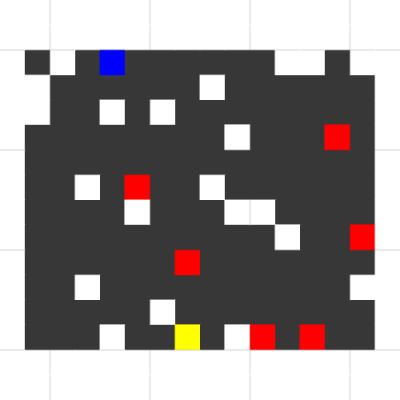
\includegraphics[width=0.5\textwidth]{ice-sliding.jpg}
  \caption{Permainan \textit{Ice Sliding Puzzle}}
  \label{fig:ice-sliding-puzzle}
\end{figure}


Tujuan akhir dari Tugas Kecil ini adalah menemukan jalur solusi yang memandu karakter utama menuju titik tujuan secara selamat. Dalam perjalanannya, pemain harus menghindari wilayah lava (kotak merah) yang akan menyebabkan \textit{game over} jika dilewati. Selain itu, terdapat modifikasi \textit{constraint} tambahan berupa \textit{tile} berangka; pemain diwajibkan untuk melewati \textit{tile} angka tersebut sesuai dengan urutan membesar secara berurutan.

\section{Dasar Teori}

\subsection{Representasi Permasalahan sebagai Graf}
Permasalahan \textit{Ice Sliding Puzzle} dapat dimodelkan sebagai masalah pencarian jalur (\textit{pathfinding}) di dalam sebuah graf ruang keadaan (\textit{state space graph}). Dalam konteks ini, graf tidak direpresentasikan secara statis di awal, melainkan dibangkitkan secara dinamis seiring dengan berjalannya eksplorasi agen. Simpul (\textit{node}) dalam graf ini merepresentasikan status atau keadaan (\textit{state}) spesifik dari permainan pada suatu waktu. Keadaan ini tidak sekadar bergantung pada letak koordinat spasial baris dan kolom agen, melainkan secara esensial mencakup parameter kemajuan \textit{checkpoint} berupa urutan angka yang telah diambil. Sisi (\textit{edge}) pada graf melambangkan transisi antar keadaan yang valid, yaitu aksi meluncur (\textit{sliding}) ke salah satu dari empat arah kardinal hingga agen berhenti akibat menabrak tembok atau rintangan. Biaya dari setiap sisi didefinisikan sebagai akumulasi biaya (\textit{cost}) dari seluruh petak yang dilalui agen selama proses meluncur dalam satu tindakan.

\subsection{Uniform Cost Search (UCS)}
Algoritma \textit{Uniform Cost Search} (UCS) merupakan algoritma pencarian tidak berinformasi (\textit{uninformed search}) yang selalu mengekspansi simpul dengan biaya lintasan kumulatif terkecil dari simpul awal. Algoritma ini menggunakan struktur data antrean prioritas (\textit{priority queue}) untuk mengurutkan daftar simpul berdasarkan nilai fungsi objektifnya. Pada simulasi \textit{Ice Sliding Puzzle}, UCS secara sekuensial akan mengekspansi arah luncuran agen, memvalidasi pergerakan (misalnya menghentikan dan menggugurkan transisi jika agen menyentuh petak lava mematikan), lalu mengakumulasi biaya pergerakan petak demi petak untuk diuji tingkat prioritasnya. 

Secara formal dalam konteks teka-teki ini, fungsi evaluasi murni dikendalikan oleh $g(n)$. Definisi dari $g(n)$ adalah total biaya traversal aktual yang dibutuhkan untuk mencapai keadaan $n$ dari posisi pijakan paling awal. Biaya akumulatif ini dikalkulasi dengan menjumlahkan \textit{cost} spesifik pada setiap ubin pijakan yang telah dilewati agen, secara eksklusif mengecualikan petak asal permulaan tolakan, namun tetap mencakup ubin dinding tempat pendaratan akhirnya berhenti bergeser. Karena algoritma terus-menerus mencari lintasan kumulatif termurah serta menyimpan
riwayat kunci kombinasi posisi dan target angka (\textit{state key}) di dalam \textit{visited map} anti-siklus, UCS terjamin menemukan rute dengan biaya paling minim selama biaya setiap sisi bernilai non negatif~[1].

\subsubsection{Langkah-Langkah Algoritma UCS}
\begin{enumerate}
\item \textbf{Inisialisasi:} Membangun sebuah antrean prioritas (\textit{priority queue}) dan memasukkan \textit{initial state} yang direpresentasikan oleh \texttt{models.GameState} berisi posisi awal aktor (\texttt{Z}) dan nilai \texttt{NextNum} yang disesuaikan dengan konfigurasi papan: bernilai \texttt{0} apabila terdapat angka pada papan, atau \texttt{-1} apabila tidak ada angka sama sekali. Biaya kumulatif awal $g = 0$ ditetapkan untuk \textit{initial state} tersebut.
\item \textbf{Struktur Perulangan:} Melakukan iterasi selama antrean prioritas tidak dalam keadaan kosong.
\item \textbf{Ekstraksi Node:} Mengambil simpul dengan total biaya aktual ($g(n)$) terkecil dari antrean prioritas untuk dievaluasi.
\item \textbf{Pengecekan Visited Set:} Memeriksa apakah kombinasi posisi koordinat dan progres \textit{checkpoint} (\texttt{NextNum}) pada simpul tersebut sudah terdapat dalam \textit{visited set}. Jika sudah pernah dikunjungi dengan biaya yang lebih rendah, maka simpul diabaikan untuk menghindari siklus tak terbatas.
\item \textbf{Uji Tujuan (\textit{Goal Test}):} Memeriksa apakah aktor telah mencapai koordinat titik keluar (\texttt{O}) dan variabel \texttt{NextNum} telah bernilai -1 (menandakan seluruh urutan angka 0--9 telah diambil). Jika terpenuhi, algoritma berhenti dan mengembalikan jalur solusi.
\item \textbf{Ekspansi dan Simulasi Meluncur:} Melakukan simulasi aksi \textit{sliding} ke empat arah kardinal. Untuk setiap arah, aktor bergerak hingga menabrak dinding (\texttt{X}) atau batas papan. Selama meluncur, biaya setiap ubin yang dilewati diakumulasikan ke dalam biaya gerak (\textit{edge cost}), kecuali ubin posisi awal gerakan tersebut.
\item \textbf{Validasi State:} Jika dalam lintasan meluncur aktor melewati petak lava (\texttt{L}) atau keluar dari batas papan tanpa menabrak rintangan, maka aksi tersebut dinyatakan gugur (\textit{invalid}). Jika valid, simpul baru dengan biaya kumulatif yang telah diperbarui dimasukkan ke dalam antrean prioritas.
\item \textbf{Terminasi:} Jika antrean kosong sebelum tujuan tercapai, algoritma berhenti dan menyatakan bahwa solusi tidak ditemukan.
\end{enumerate}

\subsection{Greedy Best-First Search (GBFS)}
Berbeda dengan UCS, \textit{Greedy Best-First Search} (GBFS) merupakan algoritma pencarian berinformasi (\textit{informed search}) yang menggunakan fungsi evaluasi:
\[
  f(n) = h(n)
\]
di mana $h(n)$ adalah estimasi biaya dari simpul $n$ menuju tujuan (\textit{goal}). GBFS sama sekali tidak mempertimbangkan biaya perjalanan yang telah ditempuh ($g(n)$ diabaikan), sehingga eksplorasi sepenuhnya dipandu oleh intuisi heuristik menuju sasaran~[1].

Dalam konteks \textit{Ice Sliding Puzzle}, GBFS pada setiap iterasi memilih arah luncuran yang menghasilkan posisi berhenti dengan nilai $h(n)$ terkecil, yaitu posisi yang diperkirakan paling dekat dengan \textit{checkpoint} berikutnya atau titik tujuan. Pendekatan ini menghasilkan kecepatan eksekusi yang tinggi karena algoritma cenderung langsung bergerak menuju sasaran. Namun, karena biaya aktual perjalanan diabaikan, GBFS tidak menjamin solusi yang optimal dan berisiko menghasilkan jalur dengan total biaya yang lebih tinggi dibanding solusi terbaik~[1].

\subsubsection{Langkah-Langkah Algoritma GBFS}
\begin{enumerate}
\item \textbf{Inisialisasi:} Memasukkan \textit{initial state} ke dalam antrean prioritas berdasarkan nilai fungsi heuristik $h(n)$ yang menghitung estimasi jarak sisa menuju tujuan atau \textit{checkpoint} berikutnya.
\item \textbf{Ekstraksi Berbasis Heuristik:} Dalam setiap iterasi, algoritma mengambil simpul yang memiliki nilai estimasi heuristik terkecil, tanpa mempertimbangkan biaya historis yang telah ditempuh.
\item \textbf{Pengecekan Duplikasi:} Menggunakan \textit{visited set} dengan kunci kombinasi posisi dan progres angka (\texttt{NextNum}) untuk memastikan algoritma tidak terjebak dalam eksplorasi berulang pada keadaan yang sama.
\item \textbf{Prosedur Meluncur:} Mensimulasikan gerakan meluncur lurus hingga aktor terhenti oleh rintangan dinding. Setiap pergerakan divalidasi terhadap keberadaan petak lava; jika aktor menyentuh lava di tengah lintasan, simpul anak tersebut tidak akan dimasukkan ke dalam daftar eksplorasi.
\item \textbf{Pembaruan Progres Checkpoint:} Jika selama gerakan meluncur aktor melewati angka yang sesuai dengan urutan target (\texttt{NextNum}), maka status \texttt{NextNum} pada simpul baru diperbarui ke angka berikutnya hingga mencapai nilai -1 setelah angka terakhir diambil.
\item \textbf{Terminasi:} Algoritma berakhir dengan sukses jika \textit{goal test} terpenuhi, atau berakhir dengan kegagalan jika seluruh ruang keadaan yang dapat dijangkau telah dieksplorasi tanpa menemukan titik tujuan.
\end{enumerate}

\subsection{A* Search (A-Star)}
Algoritma A* (\textit{A-Star}) menggabungkan keunggulan UCS dan GBFS dengan
mendefinisikan fungsi evaluasi~[2]:
\[
  f(n) = g(n) + h(n)
\]
Algoritma ini mempertimbangkan biaya aktual perjalanan sekaligus estimasi sisa biaya
menuju tujuan. Dalam konteks \textit{Ice Sliding Puzzle}, ketiga komponen fungsi
evaluasi didefinisikan sebagai berikut:
\begin{itemize}
    \item $f(n)$: estimasi total biaya solusi dari posisi awal menuju tujuan apabila
    jalur tersebut melewati simpul $n$. Simpul dengan $f(n)$ terkecil diprioritaskan
    untuk diekspansi.
    \item $g(n)$: biaya aktual kumulatif yang telah dikeluarkan untuk mencapai simpul
    $n$ dari posisi awal aktor (\texttt{Z}). Nilai ini dihitung dengan menjumlahkan
    biaya traversal seluruh petak yang telah dilalui sepanjang jalur dari awal hingga
    simpul $n$, dengan ketentuan bahwa petak posisi awal setiap gerakan tidak
    dihitung, namun petak posisi berhenti tetap dihitung.
    \item $h(n)$: estimasi biaya minimum dari simpul $n$ menuju tujuan, dihitung
    menggunakan fungsi heuristik. Nilai ini harus bersifat \textit{admissible}, yaitu
    tidak pernah melebihi biaya aktual yang sesungguhnya ($h(n) \leq h^*(n)$).
\end{itemize}
Dengan mempertahankan \textit{visited set} dan menggunakan $f(n)$ sebagai prioritas
eksplorasi, A* terjamin menemukan solusi optimal selama heuristik yang digunakan
bersifat \textit{admissible}~[2].

\subsubsection{Langkah-Langkah Algoritma A*}
\begin{enumerate}
\item \textbf{Inisialisasi:} Mempersiapkan antrean prioritas dan memasukkan simpul awal dengan nilai prioritas $f(n) = g(n) + h(n)$. Nilai $g(n)$ adalah biaya aktual (0) dan $h(n)$ adalah estimasi jarak manhattan menuju rangkaian \textit{checkpoint}.
\item \textbf{Ekstraksi Optimal:} Mengambil simpul dengan total nilai estimasi biaya terendah ($f(n)$) untuk diekspansi. Penggunaan $g(n)$ memastikan pencarian tetap memperhatikan biaya traversal ubin, sementara $h(n)$ memberikan arahan menuju tujuan.
\item \textbf{Manajemen Visited:} Mencatat setiap keadaan (\textit{posisi, NextNum}) yang telah dievaluasi. Jika simpul yang sama ditemukan kembali dengan biaya $g(n)$ yang lebih besar, simpul tersebut akan diabaikan untuk menjamin efisiensi.
\item \textbf{Mekanisme Gerakan:} Melakukan \textit{sliding} ke empat arah. Algoritma menghitung jumlah biaya (\textit{cost}) dari seluruh ubin yang dilintasi dari titik setelah keberangkatan hingga titik berhenti di depan dinding rintangan.
\item \textbf{Validasi Keamanan:} Memastikan aktor tidak melewati petak lava (\texttt{L}) dan tidak meluncur keluar dari batas arena permainan. Gerakan yang melanggar ketentuan ini dianggap tidak valid dan simpul anaknya tidak akan dibangkitkan.
\item \textbf{Goal Test dan Solusi:} Pencarian dinyatakan berhasil jika simpul yang diekstraksi berada di lokasi tujuan (\texttt{O}) dengan status seluruh angka (\textit{checkpoint}) telah terambil sesuai urutan.
\end{enumerate}

\subsection{Iterative Deepening A* (IDA*)}
\textit{Iterative Deepening A*} (IDA*) merupakan pengembangan dari algoritma A*
yang dirancang untuk mengatasi keterbatasan penggunaan memori. Algoritma A*
konvensional menyimpan seluruh simpul pada \textit{frontier} di dalam antrean
prioritas, sehingga konsumsi memori dapat tumbuh secara eksponensial pada papan
yang besar. IDA* mengatasi hal ini dengan menjalankan \textit{Depth-First Search}
(DFS) secara berulang (\textit{iterative}), dibatasi oleh nilai ambang batas
(\textit{threshold}) fungsi $f(n) = g(n) + h(n)$, tanpa memerlukan struktur data
antrean prioritas~[2].

Pada setiap iterasi, IDA* melakukan DFS rekursif dari posisi awal. Suatu cabang
pencarian dipangkas (\textit{pruning}) apabila nilai $f(n)$ pada simpul tersebut
melebihi \textit{threshold} saat ini. Apabila seluruh cabang yang dieksplorasi tidak
menghasilkan solusi, nilai \textit{threshold} diperbarui menjadi nilai $f(n)$ minimum
yang sebelumnya melampaui batas, lalu DFS dijalankan ulang dari awal. Proses ini
berlanjut hingga solusi ditemukan atau tidak ada simpul yang dapat dieksplorasi.
Dengan pendekatan ini, IDA* hanya membutuhkan memori sebesar $\mathcal{O}(bd)$ di
mana $b$ adalah \textit{branching factor} dan $d$ adalah kedalaman solusi.

\subsubsection{Langkah-Langkah Algoritma IDA*}
\begin{enumerate}
\item \textbf{Penentuan Ambang Batas Awal:} Menetapkan nilai \textit{threshold} awal yang setara dengan nilai heuristik dari posisi awal (\texttt{Z}) menuju target tujuan.
\item \textbf{Iterasi Pendalaman:} Melakukan pencarian mendalam secara rekursif (\textit{Depth-First Search}) menggunakan batasan biaya $f(n) = g(n) + h(n)$.
\item \textbf{Mekanisme Pruning:} Selama proses rekursi, jika ditemukan simpul dengan nilai $f(n)$ yang melebihi \textit{threshold} saat ini, maka cabang pencarian tersebut akan dipangkas (\textit{pruning}) dan algoritma akan kembali ke simpul sebelumnya (\textit{backtrack}).
\item \textbf{Simulasi Meluncur Rekursif:} Untuk setiap arah kardinal yang
menghasilkan gerakan valid, yaitu aktor tidak melewati petak lava dan berhenti
di depan dinding atau batas papan, algoritma melakukan transisi \textit{state}
dan mengakumulasikan biaya seluruh petak yang dilalui selama satu gerakan
\textit{sliding} untuk memperbarui nilai $g(n)$.
\item \textbf{Validasi Checkpoint:} Dalam setiap langkah rekursif, algoritma memantau apakah urutan angka 0--9 diambil secara benar. Pelanggaran urutan angka mengakibatkan status \textit{game over} dan cabang rekursi tersebut dihentikan.
\item \textbf{Pembaruan Threshold:} Jika satu iterasi penuh DFS selesai tanpa menemukan tujuan, algoritma mengidentifikasi nilai $f(n)$ terkecil yang sebelumnya melampaui \textit{threshold}. Nilai tersebut ditetapkan sebagai \textit{threshold} baru untuk iterasi berikutnya.
\item \textbf{Terminasi:} Algoritma berhenti jika tujuan ditemukan pada kedalaman tertentu. Jika setelah pembaruan \textit{threshold} nilainya mencapai tak terhingga (tidak ada lagi simpul yang dapat dievaluasi), maka algoritma berhenti dan menyatakan solusi tidak ditemukan.
\end{enumerate}

\subsection{Admissibilitas Heuristik}

Sebuah fungsi heuristik $h(n)$ dikatakan \textit{admissible} apabila untuk setiap
simpul $n$, nilai $h(n)$ tidak pernah melebihi biaya aktual minimum untuk mencapai
tujuan dari simpul tersebut, atau secara formal: $h(n) \leq h^*(n)$, di mana
$h^*(n)$ adalah biaya sesungguhnya dari $n$ ke tujuan. Heuristik yang \textit{admissible}
bersifat optimistis karena selalu meremehkan atau tepat memperkirakan biaya yang
diperlukan~[2]. Syarat ini menjamin bahwa A* dan IDA*
akan menemukan solusi yang optimal.

Berikut adalah argumen admissibilitas untuk setiap heuristik yang diimplementasikan
pada program ini:

\begin{itemize}
    \item \textbf{Heuristik 1 (H1 -- Manhattan Distance Murni):}
    H1 menghitung jarak Manhattan antara posisi aktor saat ini dengan posisi target
    (checkpoint berikutnya atau titik tujuan). Dalam permainan \textit{Ice Sliding
    Puzzle}, aktor tidak dapat bergerak diagonal dan harus meluncur hingga menabrak
    dinding. Akibatnya, jumlah petak yang sesungguhnya dilalui dalam satu jalur solusi
    selalu lebih banyak atau sama dengan jarak Manhattan antara kedua titik. Karena
    setiap petak memiliki biaya traversal minimal 1, maka $h_1(n) \leq h^*(n)$ selalu
    terpenuhi. Dengan demikian, H1 bersifat \textit{admissible}.

    \item \textbf{Heuristik 2 (H2 -- Manhattan Termodifikasi dengan MinCost dan
    Penalti Orientasi):}
    H2 menghitung estimasi biaya sebagai jarak Manhattan dikalikan dengan biaya
    traversal minimum di papan (\texttt{minCost}), ditambah penalti apabila tidak
    terdapat dinding di titik belok yang memungkinkan aktor berhenti untuk berubah
    arah. Penalti ini dikenakan karena apabila tidak ada dinding di titik belok,
    aktor dipastikan harus menempuh setidaknya satu langkah tambahan untuk dapat
    berhenti dan berbelok. Selama \texttt{minCost} adalah batas bawah biaya per
    petak yang sesungguhnya, dan penalti orientasi hanya ditambahkan ketika memang
    diperlukan secara fisik, nilai $h_2(n)$ tidak melebihi biaya aktual. Dengan
    demikian, H2 bersifat \textit{admissible}.

    \item \textbf{Heuristik 3 (H3 -- Rangkaian Manhattan Checkpoint):}
    H3 menjumlahkan jarak Manhattan secara berantai: dari posisi aktor ke
    \textit{checkpoint} berikutnya, antar setiap pasang \textit{checkpoint} yang
    tersisa, dan dari \textit{checkpoint} terakhir ke titik tujuan. Karena
    \textit{constraint} permainan mengharuskan aktor mengunjungi seluruh
    \textit{checkpoint} secara berurutan, total biaya aktual solusi pasti mencakup
    biaya menuju setiap \textit{checkpoint} tersebut. Jarak Manhattan pada setiap
    segmen merupakan batas bawah biaya segmen tersebut, sehingga penjumlahan
    seluruh segmen pun tidak melebihi biaya aktual keseluruhan jalur. Dengan
    demikian, H3 bersifat \textit{admissible}.
\end{itemize}

\subsection{Perbandingan Teoritis Algoritma}
Eksplorasi metodologis pencarian rute labirin berbasis es ini mewujudkan spektrum konsekuensi pengolahan struktur ruang masalah. Parameter pengujian keutuhan algoritma disajikan dalam ringkasan komparasi formal pada Tabel \ref{tab:perbandingan}.

\begin{table}[H]
    \centering
    \caption{Perbandingan Teoretis Algoritma Pencarian \textit{Pathfinding}}
    \label{tab:perbandingan}
    \begin{threeparttable}
        \begin{tabular}{lcccc}
            \toprule
            \textbf{Algoritma} & \textbf{\textit{Complete}} & \textbf{Optimal} & \textbf{Waktu} & \textbf{Memori} \\
            \midrule
            UCS   & Ya  & Ya       & $\mathcal{O}(b^{1+\lfloor C^*/\epsilon \rfloor})$ & $\mathcal{O}(b^{1+\lfloor C^*/\epsilon \rfloor})$ \\
            GBFS  & Ya* & Tidak    & $\mathcal{O}(b^m)$ & $\mathcal{O}(b^m)$ \\
            A*    & Ya  & Ya\tnote{a} & $\mathcal{O}(b^d)$ & $\mathcal{O}(b^d)$ \\
            IDA*  & Ya  & Ya\tnote{a} & $\mathcal{O}(b^d)$ & $\mathcal{O}(bd)$ \\
            \bottomrule
        \end{tabular}
        \begin{tablenotes}
            \footnotesize
            \item[a] Dijamin optimal apabila fungsi heuristik $h(n)$ bersifat \textit{admissible}.
            \item[*] \textit{Complete} dengan syarat terdapat \textit{visited set} untuk mencegah siklus.
        \end{tablenotes}
    \end{threeparttable}
\end{table}

Secara teoritis, setiap algoritma menunjukkan karakteristik yang berbeda dalam
konteks \textit{Ice Sliding Puzzle}. \textbf{UCS} menjamin kelengkapan dan
optimalitas pencarian, namun mengeksplorasi simpul secara merata ke seluruh arah
tanpa panduan menuju tujuan. Hal ini menyebabkan jumlah simpul yang diekspansi
cenderung besar, terutama pada papan yang luas, sehingga konsumsi waktu dan memori
menjadi tinggi~[1].

\textbf{GBFS} berkebalikan dengan UCS: algoritma ini cepat menemukan suatu solusi
karena seluruh eksplorasi dipandu oleh heuristik menuju tujuan. Namun, karena biaya
aktual perjalanan sepenuhnya diabaikan, solusi yang ditemukan tidak dijamin optimal
dan algoritma dapat menghasilkan jalur dengan total biaya yang jauh lebih tinggi
dari solusi terbaik~[1].

\textbf{A*} menyeimbangkan kedua pendekatan di atas. Dengan mempertimbangkan $g(n)$
dan $h(n)$ secara bersamaan, A* mampu menemukan solusi optimal dengan jumlah
eksplorasi simpul yang lebih sedikit dibanding UCS, selama heuristik yang digunakan
bersifat \textit{admissible}. Kelemahan A* terletak pada penggunaan memori yang
tetap tinggi karena seluruh simpul pada \textit{frontier} harus disimpan dalam
antrean prioritas~[2].

\textbf{IDA*} mengatasi keterbatasan memori A* dengan mengganti antrean prioritas
dengan DFS rekursif berbasis \textit{threshold}. Memori yang digunakan hanya
$\mathcal{O}(bd)$, jauh lebih efisien dibanding A*. Konsekuensinya, IDA*
kemungkinan mengekspansi simpul yang sama beberapa kali di iterasi yang berbeda,
sehingga waktu eksekusinya dapat lebih lambat dari A* pada beberapa kasus tertentu.

\section{Desain dan Implementasi}

Logika pergerakan agen dalam permainan ini sangat bergantung pada desain ruang status (\textit{state space}). Dalam implementasinya menggunakan bahasa Go, status agen direpresentasikan melalui struktur \texttt{GameState}. Karena aturan permainan mewajibkan agen untuk mengambil seluruh angka sebelum menuju titik akhir, definisi status tidak hanya menyimpan koordinat lokasi, tetapi juga target angka selanjutnya.

Koordinat spasial agen disimpan dalam atribut \texttt{Pos} bertipe \texttt{Position} yang merepresentasikan baris dan kolom. Sementara itu, atribut \texttt{NextNum} bertipe \texttt{int} berfungsi untuk melacak target angka yang sedang dicari oleh agen saat ini. Jika \texttt{NextNum} bernilai -1, hal ini menandakan bahwa seluruh angka telah berhasil dikumpulkan, sehingga \textit{goal test} dapat dievaluasi.

Penggabungan kedua atribut tersebut ke dalam \textit{StateKey} bertujuan untuk mencegah terjadinya \textit{false-positive} pada \textit{visited set}. Dengan rancangan ini, agen yang telah mengambil suatu angka lalu kembali melewati koordinat yang sama tidak akan dideteksi sebagai \textit{looping} (jalan buntu). Adanya perubahan nilai pada \texttt{NextNum} membuat kondisi tersebut dikenali sebagai status (\textit{state}) baru yang valid menuju tujuan akhir.

\subsection{Simulasi Gerakan Sliding}

Berbeda dari permasalahan pencarian jalur pada umumnya di mana satu aksi
merepresentasikan perpindahan ke satu petak tetangga, dalam \textit{Ice Sliding
Puzzle} satu aksi merepresentasikan satu gerakan meluncur penuh hingga berhenti.
Fungsi simulasi sliding dijalankan secara iteratif dalam sebuah perulangan, di mana
posisi aktor diperbarui satu petak per iterasi ke arah yang dipilih hingga kondisi
berhenti terpenuhi. Berikut adalah langkah-langkah yang dilakukan dalam satu
simulasi gerakan sliding:

\begin{enumerate}
    \item \textbf{Translasi Posisi:} Pada setiap iterasi perulangan, posisi aktor
    diperbarui satu petak ke arah yang dipilih (atas, bawah, kiri, atau kanan)
    dengan menambahkan delta baris atau kolom yang sesuai.

    \item \textbf{Pemeriksaan Batas Papan (\textit{Bounds Checking}):} Apabila
    posisi baru berada di luar batas papan dan tidak ada dinding yang menghentikan
    aktor, gerakan tersebut dinyatakan tidak valid (\textit{game over}) dan aksi
    sliding ini digugurkan.

    \item \textbf{Deteksi Lava:} Apabila petak yang akan dimasuki bertipe lava
    (\texttt{TileLava}), gerakan dinyatakan tidak valid karena melewati lava
    menyebabkan \textit{game over}. Aksi sliding ini digugurkan sepenuhnya.

    \item \textbf{Deteksi Dinding dan Kondisi Berhenti:} Apabila petak di depan
    aktor (satu langkah lebih jauh dalam arah gerak) bertipe dinding
    (\texttt{TileWall}), aktor berhenti di petak saat ini. Perulangan dihentikan
    dan posisi ini menjadi posisi berhenti yang valid.

    \item \textbf{Akumulasi Biaya Traversal:} Biaya traversal petak yang baru
    dimasuki (diambil dari \texttt{m.CostAt(currPos)}) ditambahkan ke total biaya
    gerakan. Petak posisi awal gerakan tidak dihitung, sedangkan petak posisi
    berhenti tetap dihitung.

    \item \textbf{Pembaruan Progres Checkpoint:} Apabila petak yang baru dimasuki
    merupakan \textit{checkpoint} bernomor dan nomornya sesuai dengan \texttt{NextNum}
    saat ini, nilai \texttt{NextNum} diperbarui ke angka berikutnya. Apabila aktor
    melewati angka yang tidak sesuai urutan, aksi sliding digugurkan karena melanggar
    aturan permainan.
\end{enumerate}

\subsection{Desain Heuristik}
Program mengimplementasikan tiga fungsi heuristik dengan tingkat kompleksitas yang
berbeda-beda. Ketiga heuristik dirancang untuk memenuhi syarat \textit{admissible},
sehingga dapat menjamin optimalitas solusi ketika digunakan pada algoritma A* dan
IDA*.

Heuristik pertama (H1) menghitung jarak Manhattan dari posisi aktor saat ini ke
posisi tujuan (atau \textit{checkpoint} berikutnya apabila masih ada). Ini merupakan
estimasi paling sederhana dan selalu bersifat \textit{admissible}:
\begin{lstlisting}[style=go]
// Heuristic1 mengimplementasikan Manhattan Murni (jarak langsung ke tujuan).
func Heuristic1(state *models.GameState, m *models.MapData) int {
	return manhattanDistance(state.Pos, m.GoalPos)
}
\end{lstlisting}

Heuristik kedua (H2) memodifikasi H1 dengan mengalikan jarak Manhattan dengan biaya
traversal minimum yang terdapat di papan (\texttt{m.MinCost}), sehingga estimasi
mencerminkan biaya aktual minimum per petak. Selain itu, H2 menambahkan penalti
apabila tidak terdapat dinding di titik belok yang diperlukan, mengindikasikan
bahwa aktor kemungkinan harus menempuh langkah tambahan untuk dapat berbelok arah:
\begin{lstlisting}[style=go]
// Heuristic2 mengimplementasikan Manhattan termodifikasi dengan faktor minCost.
func Heuristic2(state *models.GameState, m *models.MapData) int {
	baseDist := manhattanDistance(state.Pos, m.GoalPos)
	penalty := 0
	if m.Grid[m.GoalPos.X][state.Pos.Y] != models.TileWall && 
	   m.Grid[state.Pos.X][m.GoalPos.Y] != models.TileWall {
		penalty = m.MinCost
	}
	return (baseDist * m.MinCost) + penalty
}
\end{lstlisting}

Heuristik ketiga (H3) dirancang untuk papan yang memiliki \textit{constraint}
angka berurutan. H3 menjumlahkan jarak Manhattan secara berantai: dari posisi
aktor ke \textit{checkpoint} berikutnya, antar setiap pasang \textit{checkpoint}
yang tersisa, hingga dari \textit{checkpoint} terakhir ke titik tujuan. Apabila
tidak ada angka yang tersisa, H3 berperilaku identik dengan H1:
\begin{lstlisting}[style=go]
// Heuristic3 mengimplementasikan Manhattan Checkpoint Berantai.
func Heuristic3(state *models.GameState, m *models.MapData) int {
	if state.NextNum == -1 {
		return manhattanDistance(state.Pos, m.GoalPos)
	}
	cost := 0
	// 1. Jarak ke target angka pertama
	cost += manhattanDistance(state.Pos, m.NumberPos[state.NextNum])
	// 2. Jarak berantai antar sisa angka yang belum terkumpul
	for i := state.NextNum; i < m.TotalNumbers-1; i++ {
		cost += manhattanDistance(m.NumberPos[i], m.NumberPos[i+1])
	}
	// 3. Jarak angka terakhir ke titik keluar
	if m.TotalNumbers > 0 {
		cost += manhattanDistance(m.NumberPos[m.TotalNumbers-1], m.GoalPos)
	}
	return cost
}
\end{lstlisting}

\subsection{Arsitektur Program}
Arsitektur program mengikuti pola \textit{layered architecture} dengan pemisahan yang jelas antara lapisan data, logika pencarian, dan antarmuka pengguna. Seluruh kode ditulis dalam bahasa Go dan dibagi ke dalam beberapa \textit{package} modular sesuai dengan tanggung jawabnya masing-masing (\textit{separation of concerns}):
\begin{itemize}
    \item \textbf{Package \texttt{models}:} Mendefinisikan seluruh struktur data
    inti yang digunakan bersama oleh komponen lain. Mencakup \texttt{MapData}
    (representasi papan, grid tile, dan matriks biaya), \texttt{GameState} (posisi
    aktor dan progres \textit{checkpoint}), \texttt{Position}, \texttt{Direction},
    \texttt{SolverResult} (hasil pencarian beserta statistik), dan \texttt{SearchFrame}
    (potret status ekspansi untuk keperluan visualisasi).

    \item \textbf{Package \texttt{parser}:} Bertanggung jawab membaca dan memvalidasi
    file konfigurasi papan berformat \texttt{.txt}. Paket ini memvalidasi keberadaan
    tepat satu titik awal (\texttt{Z}) dan satu titik tujuan (\texttt{O}), memastikan
    angka-angka pada papan berurutan mulai dari 0, serta memisahkan lapisan grid
    tile dan matriks biaya traversal.

    \item \textbf{Package \texttt{solver}:} Berisi implementasi keempat algoritma
    pencarian: UCS (\texttt{ucs.go}), GBFS (\texttt{gbfs.go}), A* (\texttt{astar.go}),
    dan IDA* (\texttt{idastar.go}), serta fungsi-fungsi heuristik (\texttt{heuristics.go})
    dan implementasi \textit{priority queue} berbasis \texttt{container/heap}
    (\texttt{pq.go}). Setiap algoritma mencatat \texttt{SearchFrame} selama proses
    ekspansi simpul untuk keperluan visualisasi pada GUI.

    \item \textbf{Package \texttt{gui}:} Mengimplementasikan antarmuka pengguna
    grafis menggunakan \textit{framework} Fyne v2. Komponen \texttt{BoardRenderer}
    menangani visualisasi papan dan jalur solusi, \texttt{LeftPanel} menyediakan
    kontrol algoritma dan \textit{playback}, serta \texttt{ViewState} mengelola
    status tampilan dua fase (fase pencarian dan fase solusi).
\end{itemize}

\subsection{Struktur Proyek}
    
    Struktur proyek disusun sedemikian rupa sehingga ada pemisahan antara 2 komponen utama aplikasi, yaitu folder \texttt{core} yang mengandung modul \textit{parsing}, struktur data, dan \textit{solver} berdasarkan masing-masing algoritma \textit{pathfinding} serta \texttt{gui} yang mengandung modul antarmuka grafis untuk visualisasi aplikasi. 

\begin{lstlisting}[style=bash, caption={Struktur direktori proyek}]
Tucil3_13524037_13524056/
+-- bin/
|   +-- tucil3                      # Binary hasil kompilasi
+-- doc/
|   +-- main.tex                    # Sumber laporan LaTeX
|   +-- main.pdf                    # Laporan dalam PDF
|   +-- ice-sliding.jpg             
|   +-- logo-itb.png               
+-- src/
|   +-- go.mod
|   +-- go.sum
|   +-- main.go                     # Titik masuk program
|   +-- core/
|   |   +-- models/                 # Struktur data inti
|   |   |   +-- direction.go
|   |   |   +-- map.go
|   |   |   +-- position.go
|   |   |   +-- solver.go
|   |   |   +-- state.go
|   |   +-- parser/
|   |   |   +-- parser.go
|   |   +-- solver/
|   |       +-- astar.go        # Algoritma A*
|   |       +-- gbfs.go         # Greedy Best-First Search
|   |       +-- heuristics.go   # H1, H2, H3
|   |       +-- idastar.go      # Iterative Deepening A*
|   |       +-- pq.go           # PriorityQueue
|   |       +-- ucs.go          # Uniform Cost Search
|   +-- gui/
|       +-- boardrenderer.go
|       +-- leftpanel.go
|       +-- viewstate.go
|       +-- window.go
+-- test/
    +-- input/                  # Test case
    +-- output/                 # Output solusi
\end{lstlisting}


\section{Eksperimen dan Hasil Pengujian}

Pada bagian ini, dilakukan pengujian terhadap keempat algoritma pencarian (UCS, GBFS, A*, dan IDA*) menggunakan empat konfigurasi test case dengan profil berbeda.

\subsection{Konfigurasi Test Case}

Berikut adalah profil dari file test case yang digunakan:

\begin{table}[H]
    \centering
    \caption{Profil Test Case}
    \label{tab:testcase-profile}
    \begin{tabular}{|c|l|p{8cm}|}
        \hline
        \textbf{Test Case} & \textbf{Nama File} & \textbf{Profil} \\
        \hline
        TC1 (UCS) & input1.txt & Board 7$\times$9, cost sangat bervariasi (1--9), tidak ada checkpoint/lava. UCS terpaksa mengeksplorasi banyak kombinasi cost sebelum menemukan jalur optimal. \\
        \hline
        TC2 (GBFS) & input2.txt & Board 9$\times$7, semua cost seragam (=1), banyak rintangan X berbentuk zigzag. Dengan cost seragam, perbedaan UCS vs GBFS murni pada strategi eksplorasi. \\
        \hline
        TC3 (A*/IDA*) & input3.txt & Board 9$\times$9, ada checkpoint 0$\rightarrow$1$\rightarrow$2 dan lava. Kasus utama untuk menunjukkan H3 $>$ H2 $>$ H1. \\
        \hline
        TC4 (Stress) & input4.txt & Board 11$\times$11, checkpoint 0$\rightarrow$1$\rightarrow$2$\rightarrow$3 tersebar di area berbeda + lava. Perbedaan node yang dieksplorasi H1 vs H3 sangat dramatis. \\
        \hline
    \end{tabular}
\end{table}

\subsection{UCS (Uniform Cost Search)}

\subsubsection{UCS dengan input1.txt}

\begin{figure}[H]
  \centering
  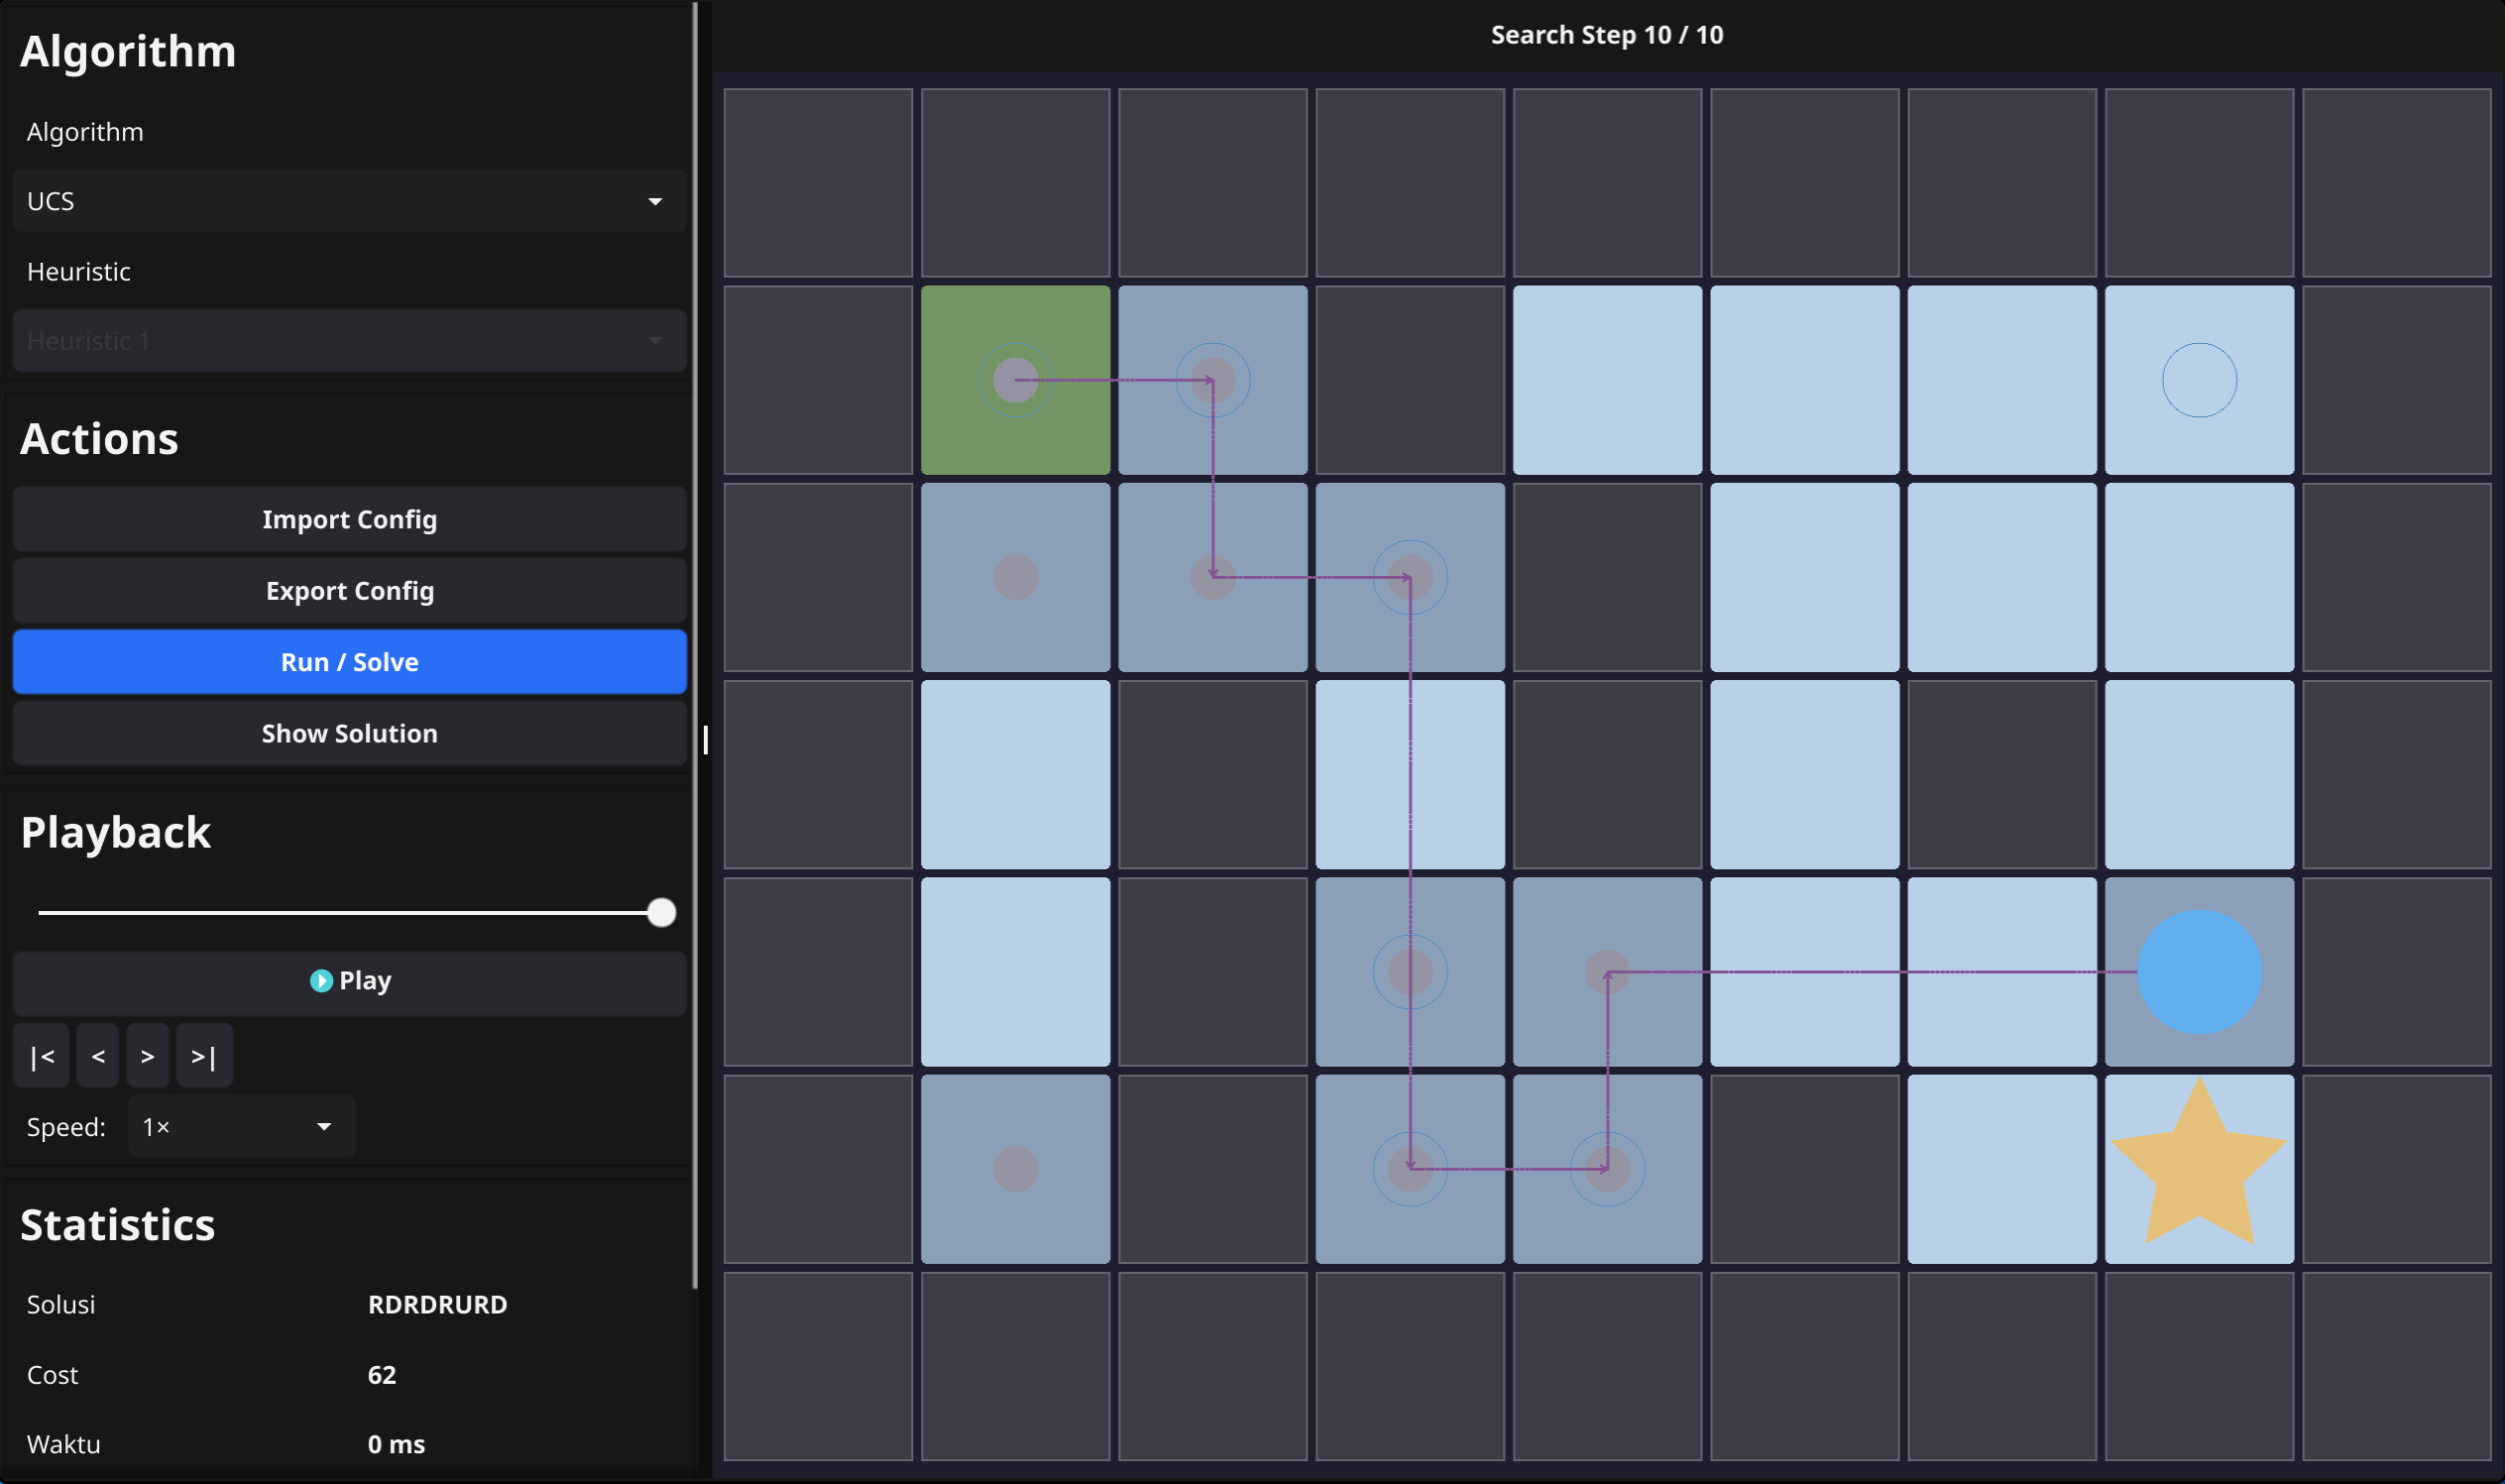
\includegraphics[width=0.8\textwidth]{ucs.png}
  \caption{Hasil UCS dengan input1.txt}
\end{figure}

\begin{tcolorbox}[title=\textbf{Hasil Pengujian}, colback=green!5!white, colframe=green!50!black]
\textbf{Solusi:} RDRDRURD\\
\textbf{Cost:} 62\\
\textbf{Waktu:} 0 ms\\
\textbf{Iterasi:} 12
\end{tcolorbox}

\subsection{GBFS (Greedy Best-First Search)}

\subsubsection{GBFS Heuristik 1 dengan input2.txt}

\begin{figure}[H]
  \centering
  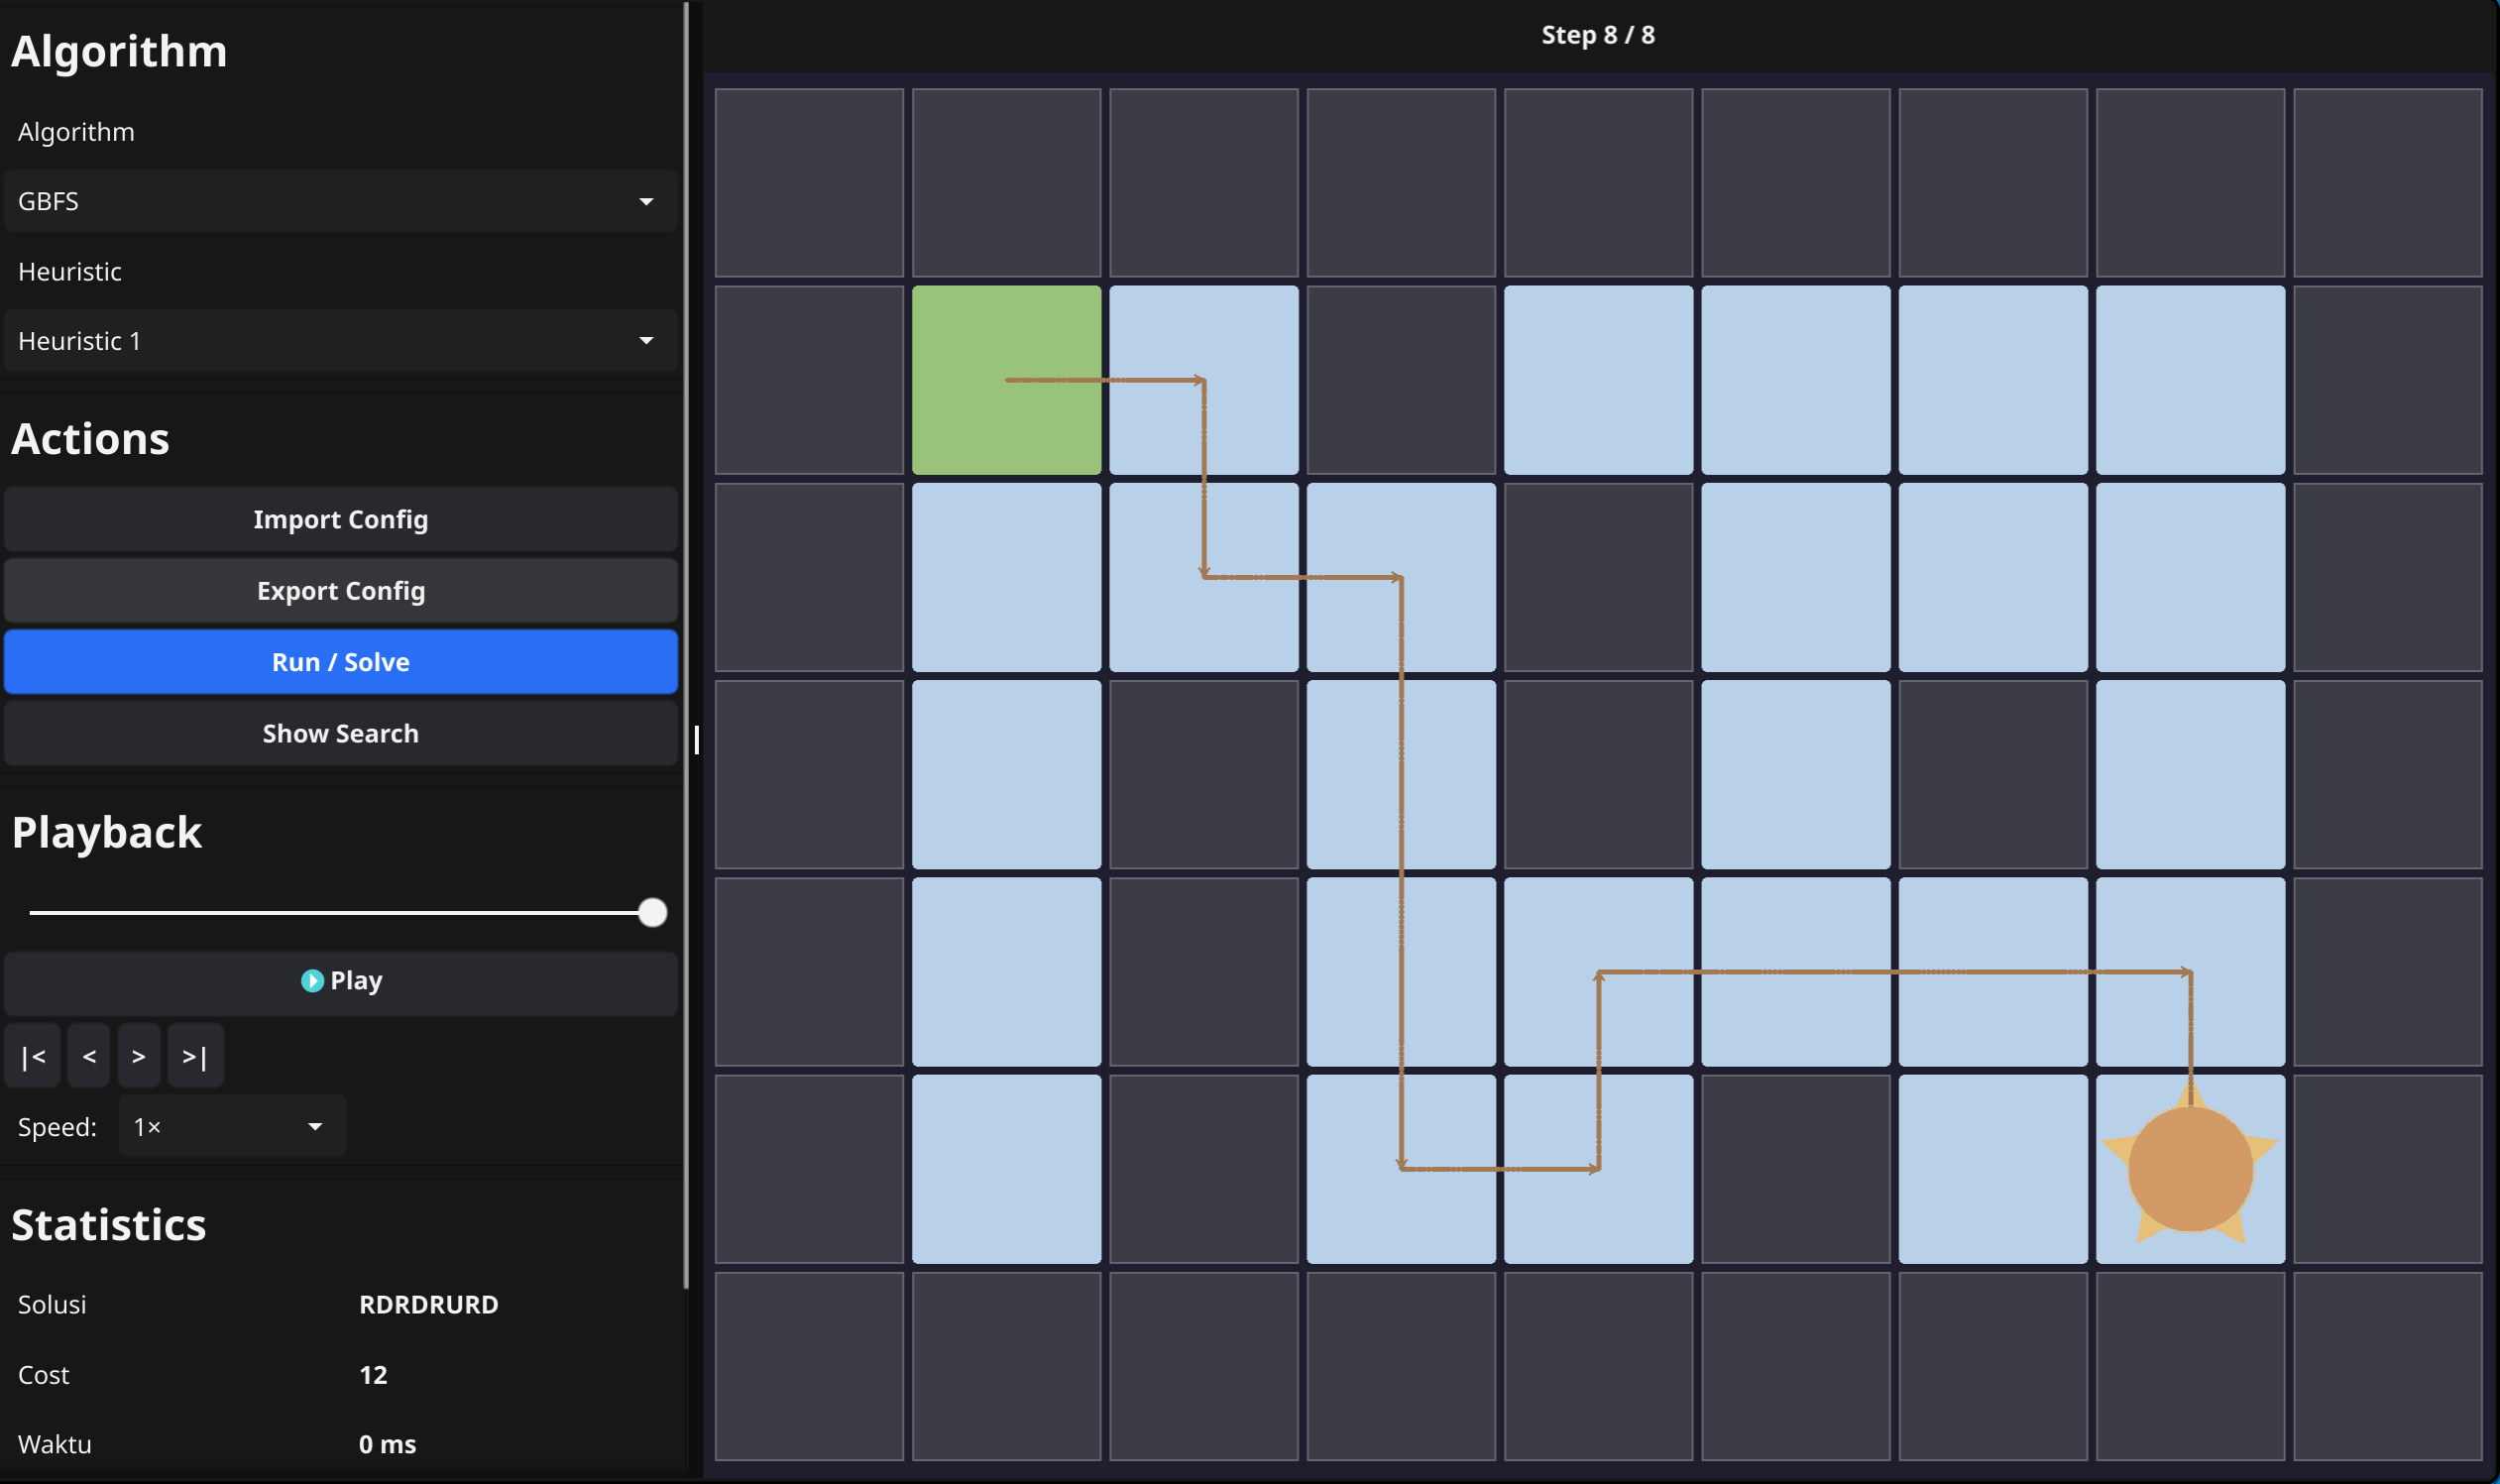
\includegraphics[width=0.8\textwidth]{gbfs_1.png}
  \caption{Hasil GBFS Heuristik 1 dengan input2.txt}
\end{figure}

\begin{tcolorbox}[title=\textbf{Hasil Pengujian}, colback=green!5!white, colframe=green!50!black]
\textbf{Solusi:} RDRDRURD\\
\textbf{Cost:} 12\\
\textbf{Waktu:} 0 ms\\
\textbf{Iterasi:} 10
\end{tcolorbox}

\subsubsection{GBFS Heuristik 2 dengan input2.txt}

\begin{figure}[H]
  \centering
  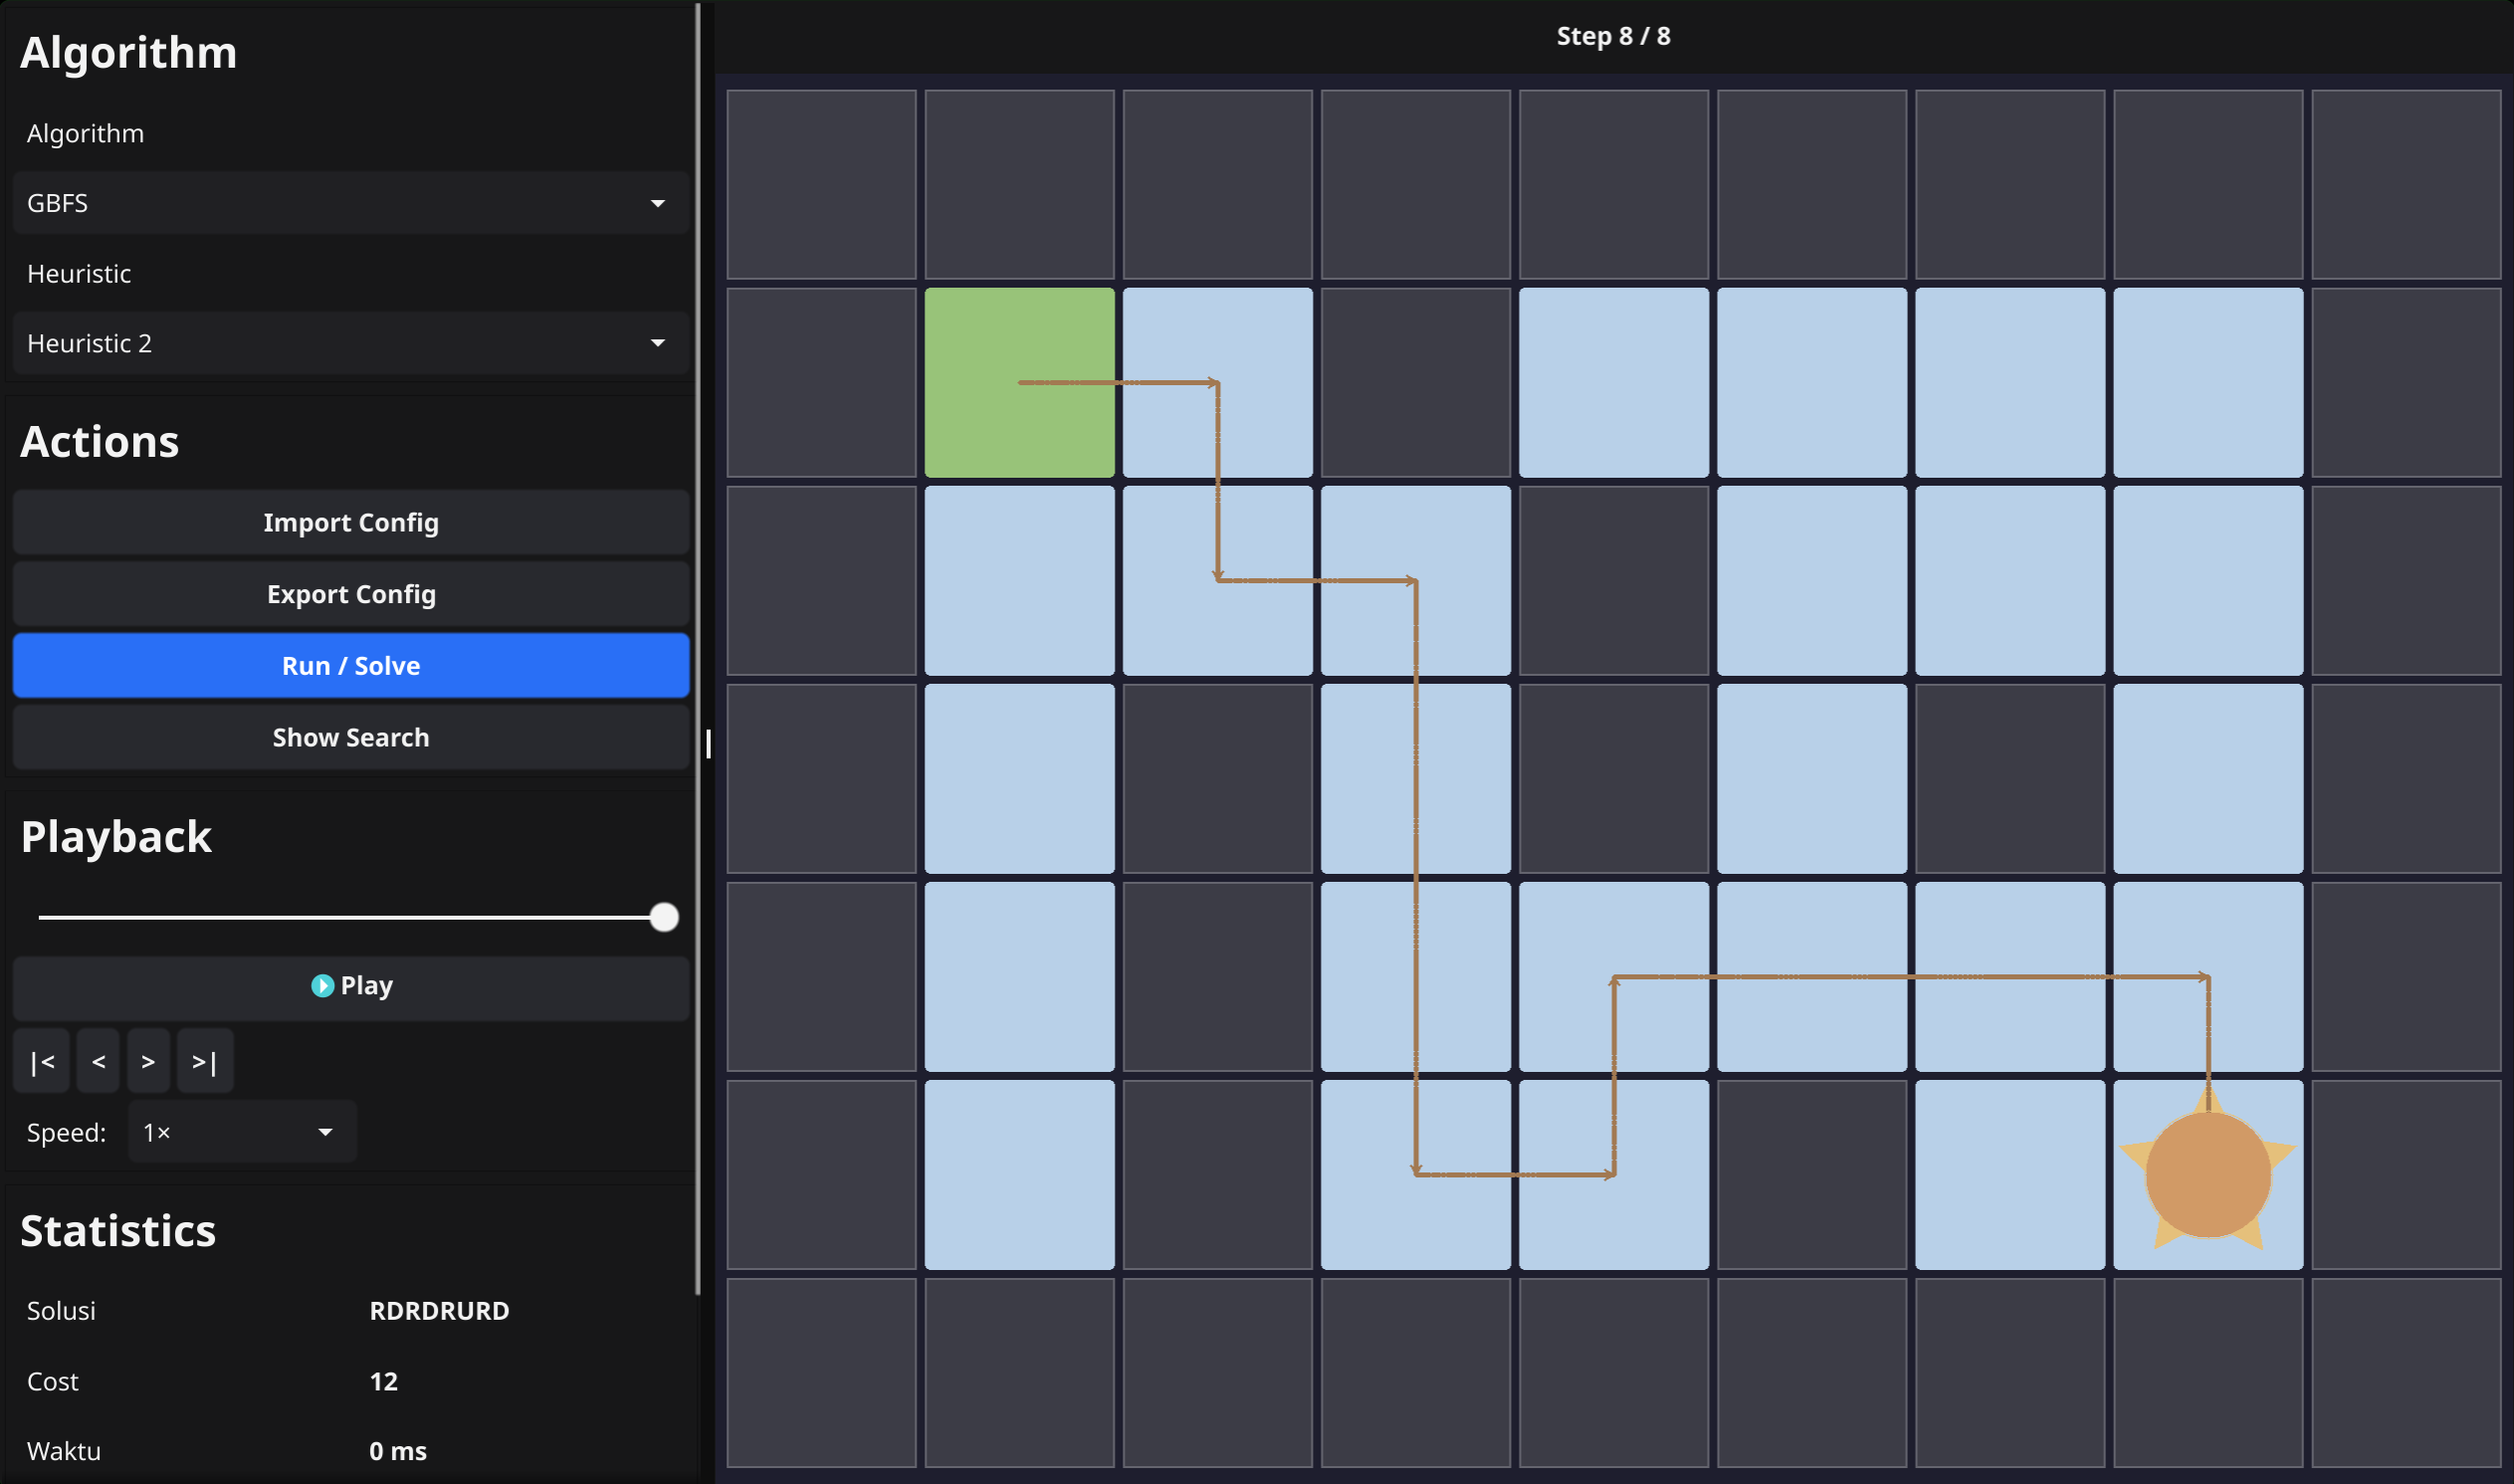
\includegraphics[width=0.8\textwidth]{gbfs_2.png}
  \caption{Hasil GBFS Heuristik 2 dengan input2.txt}
\end{figure}

\begin{tcolorbox}[title=\textbf{Hasil Pengujian}, colback=green!5!white, colframe=green!50!black]
\textbf{Solusi:} RDRDRURD\\
\textbf{Cost:} 12\\
\textbf{Waktu:} 0 ms\\
\textbf{Iterasi:} 10
\end{tcolorbox}

\subsubsection{GBFS Heuristik 3 dengan input2.txt}

\begin{figure}[H]
  \centering
  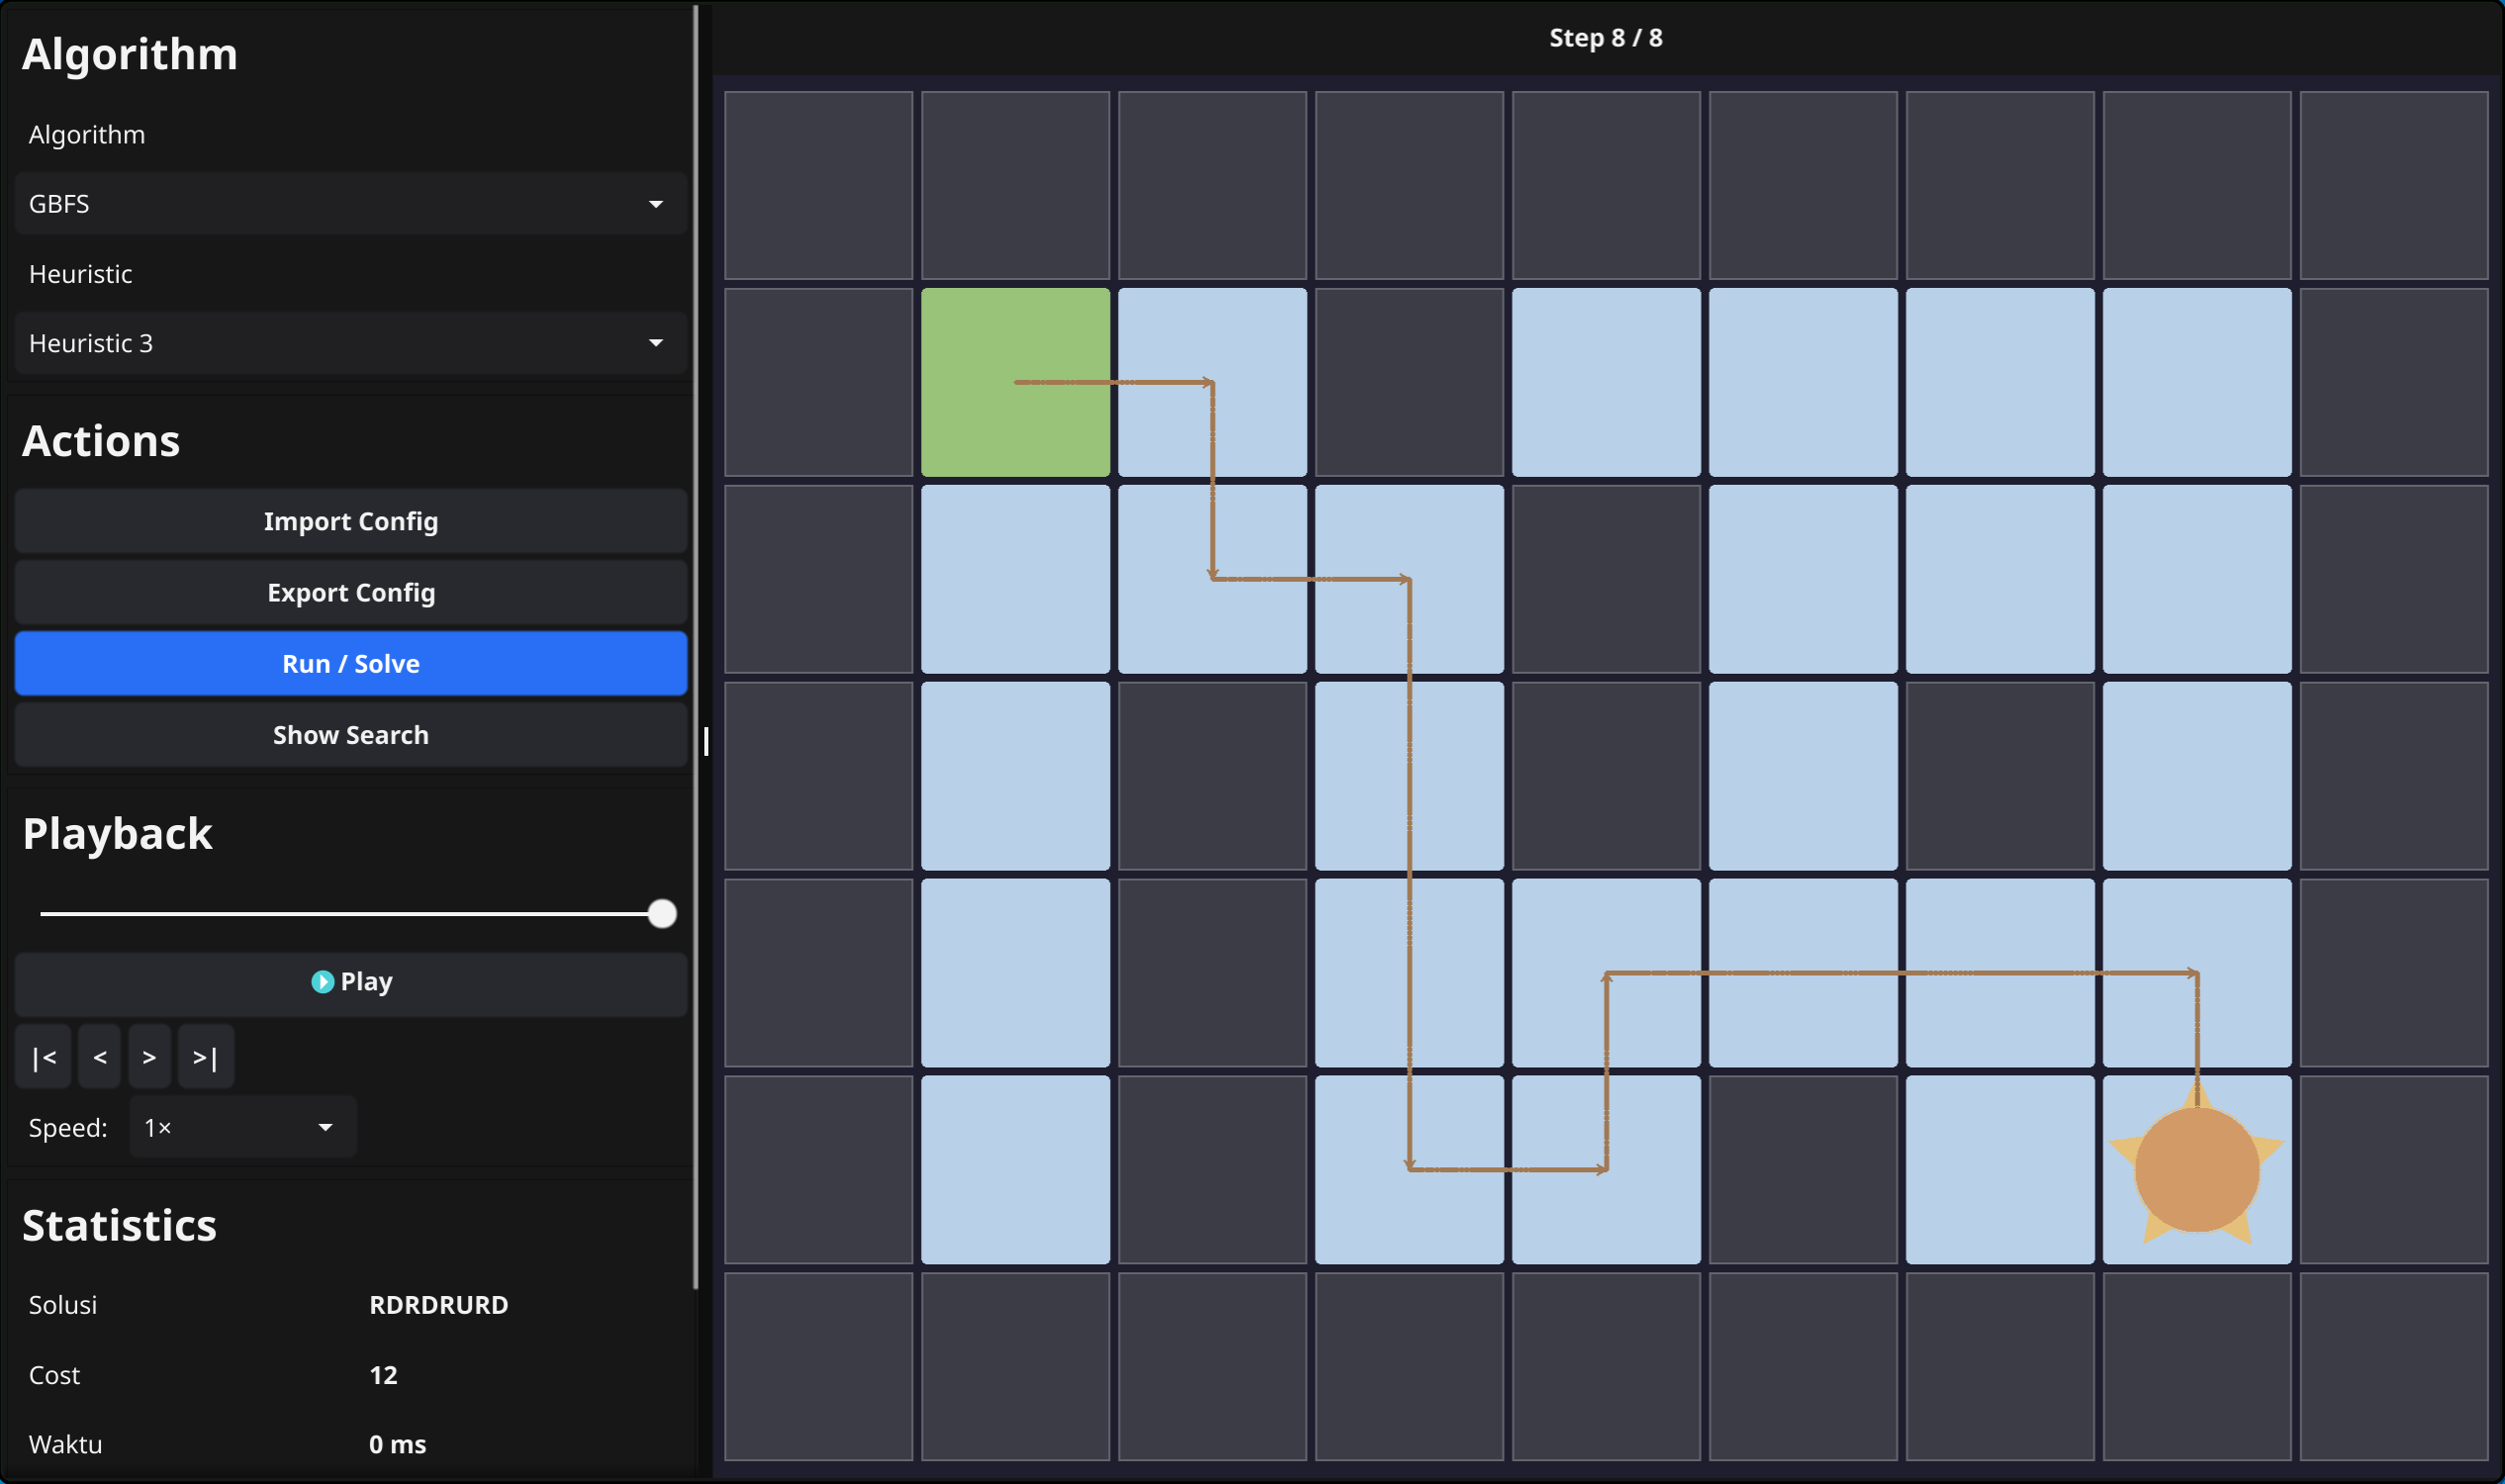
\includegraphics[width=0.8\textwidth]{gbfs_3.png}
  \caption{Hasil GBFS Heuristik 3 dengan input2.txt}
\end{figure}

\begin{tcolorbox}[title=\textbf{Hasil Pengujian}, colback=green!5!white, colframe=green!50!black]
\textbf{Solusi:} RDRDRURD\\
\textbf{Cost:} 12\\
\textbf{Waktu:} 0 ms\\
\textbf{Iterasi:} 10
\end{tcolorbox}

\subsection{A* Search dengan input3.txt}

\subsubsection{A* Heuristik 1 dengan input3.txt}

\begin{figure}[H]
  \centering
  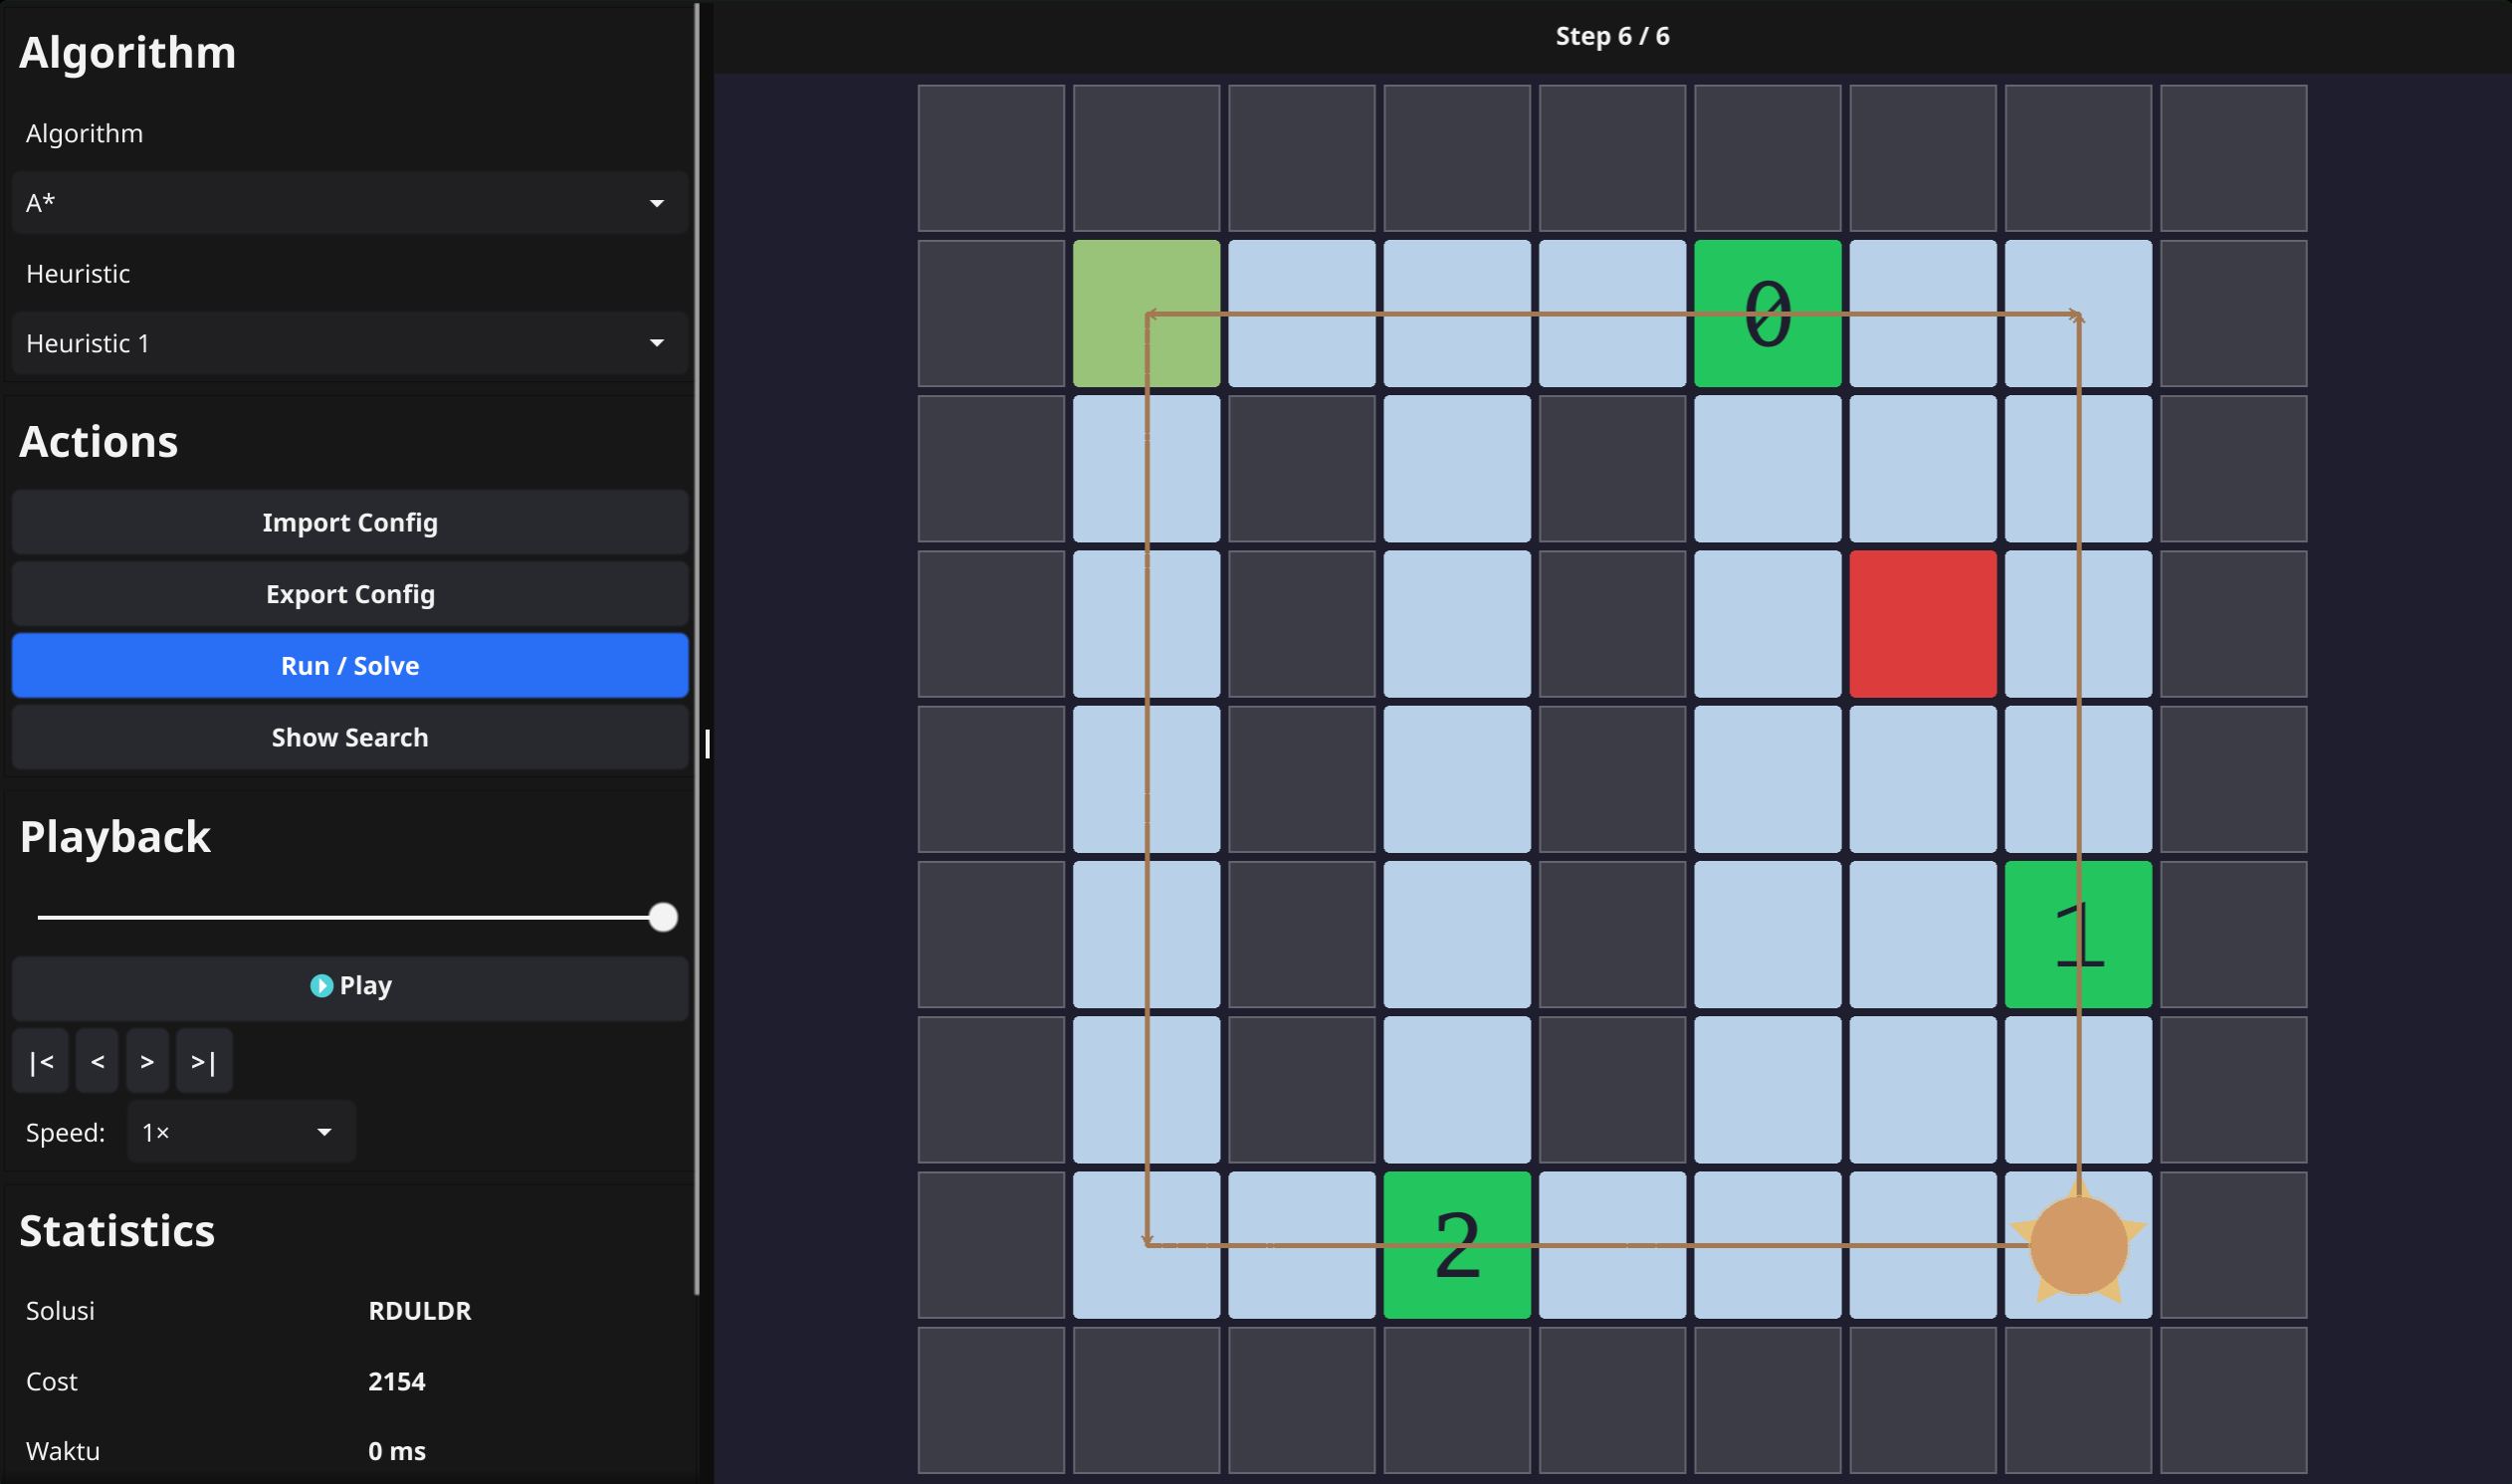
\includegraphics[width=0.8\textwidth]{astar_1.png}
  \caption{Hasil A* Heuristik 1 dengan input3.txt}
\end{figure}

\begin{tcolorbox}[title=\textbf{Hasil Pengujian}, colback=green!5!white, colframe=green!50!black]
\textbf{Solusi:} RDULDR\\
\textbf{Cost:} 2154\\
\textbf{Waktu:} 0 ms\\
\textbf{Iterasi:} 12
\end{tcolorbox}

\subsubsection{A* Heuristik 2 dengan input3.txt}

\begin{figure}[H]
  \centering
  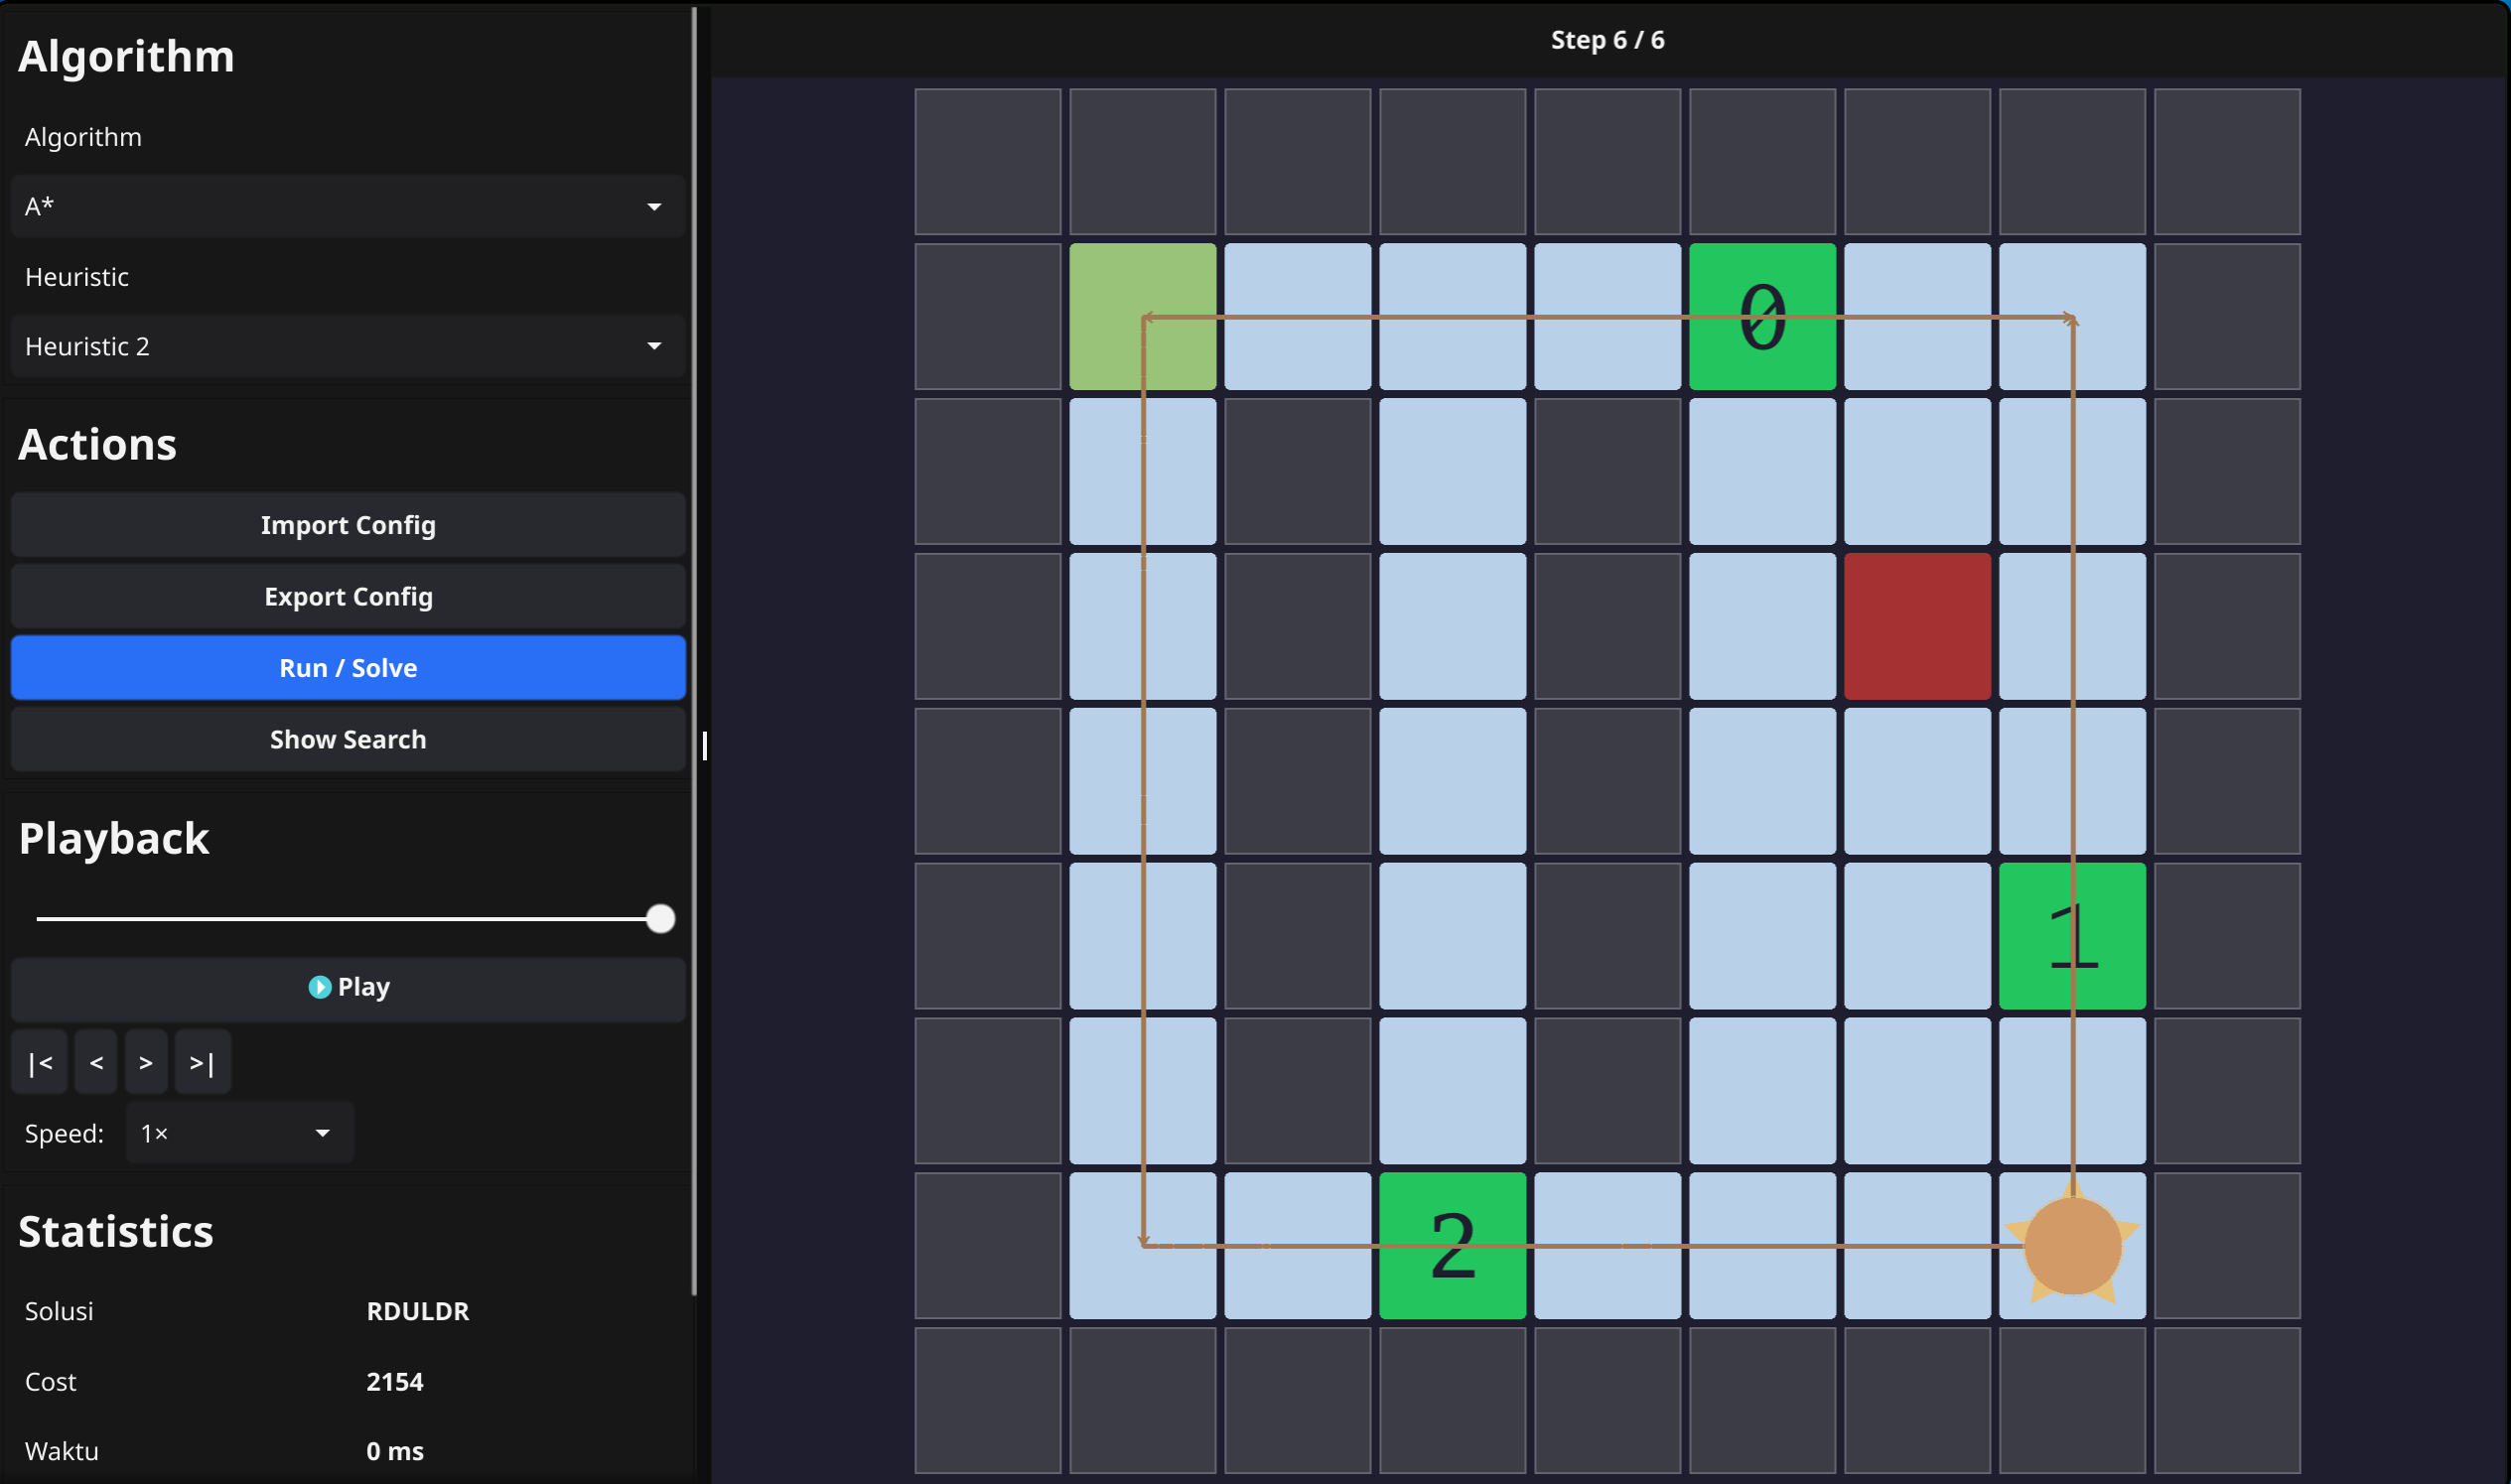
\includegraphics[width=0.8\textwidth]{astar_2.png}
  \caption{Hasil A* Heuristik 2 dengan input3.txt}
\end{figure}

\begin{tcolorbox}[title=\textbf{Hasil Pengujian}, colback=green!5!white, colframe=green!50!black]
\textbf{Solusi:} RDULDR\\
\textbf{Cost:} 2154\\
\textbf{Waktu:} 0 ms\\
\textbf{Iterasi:} 12
\end{tcolorbox}

\subsubsection{A* Heuristik 3 dengan input3.txt}

\begin{figure}[H]
  \centering
  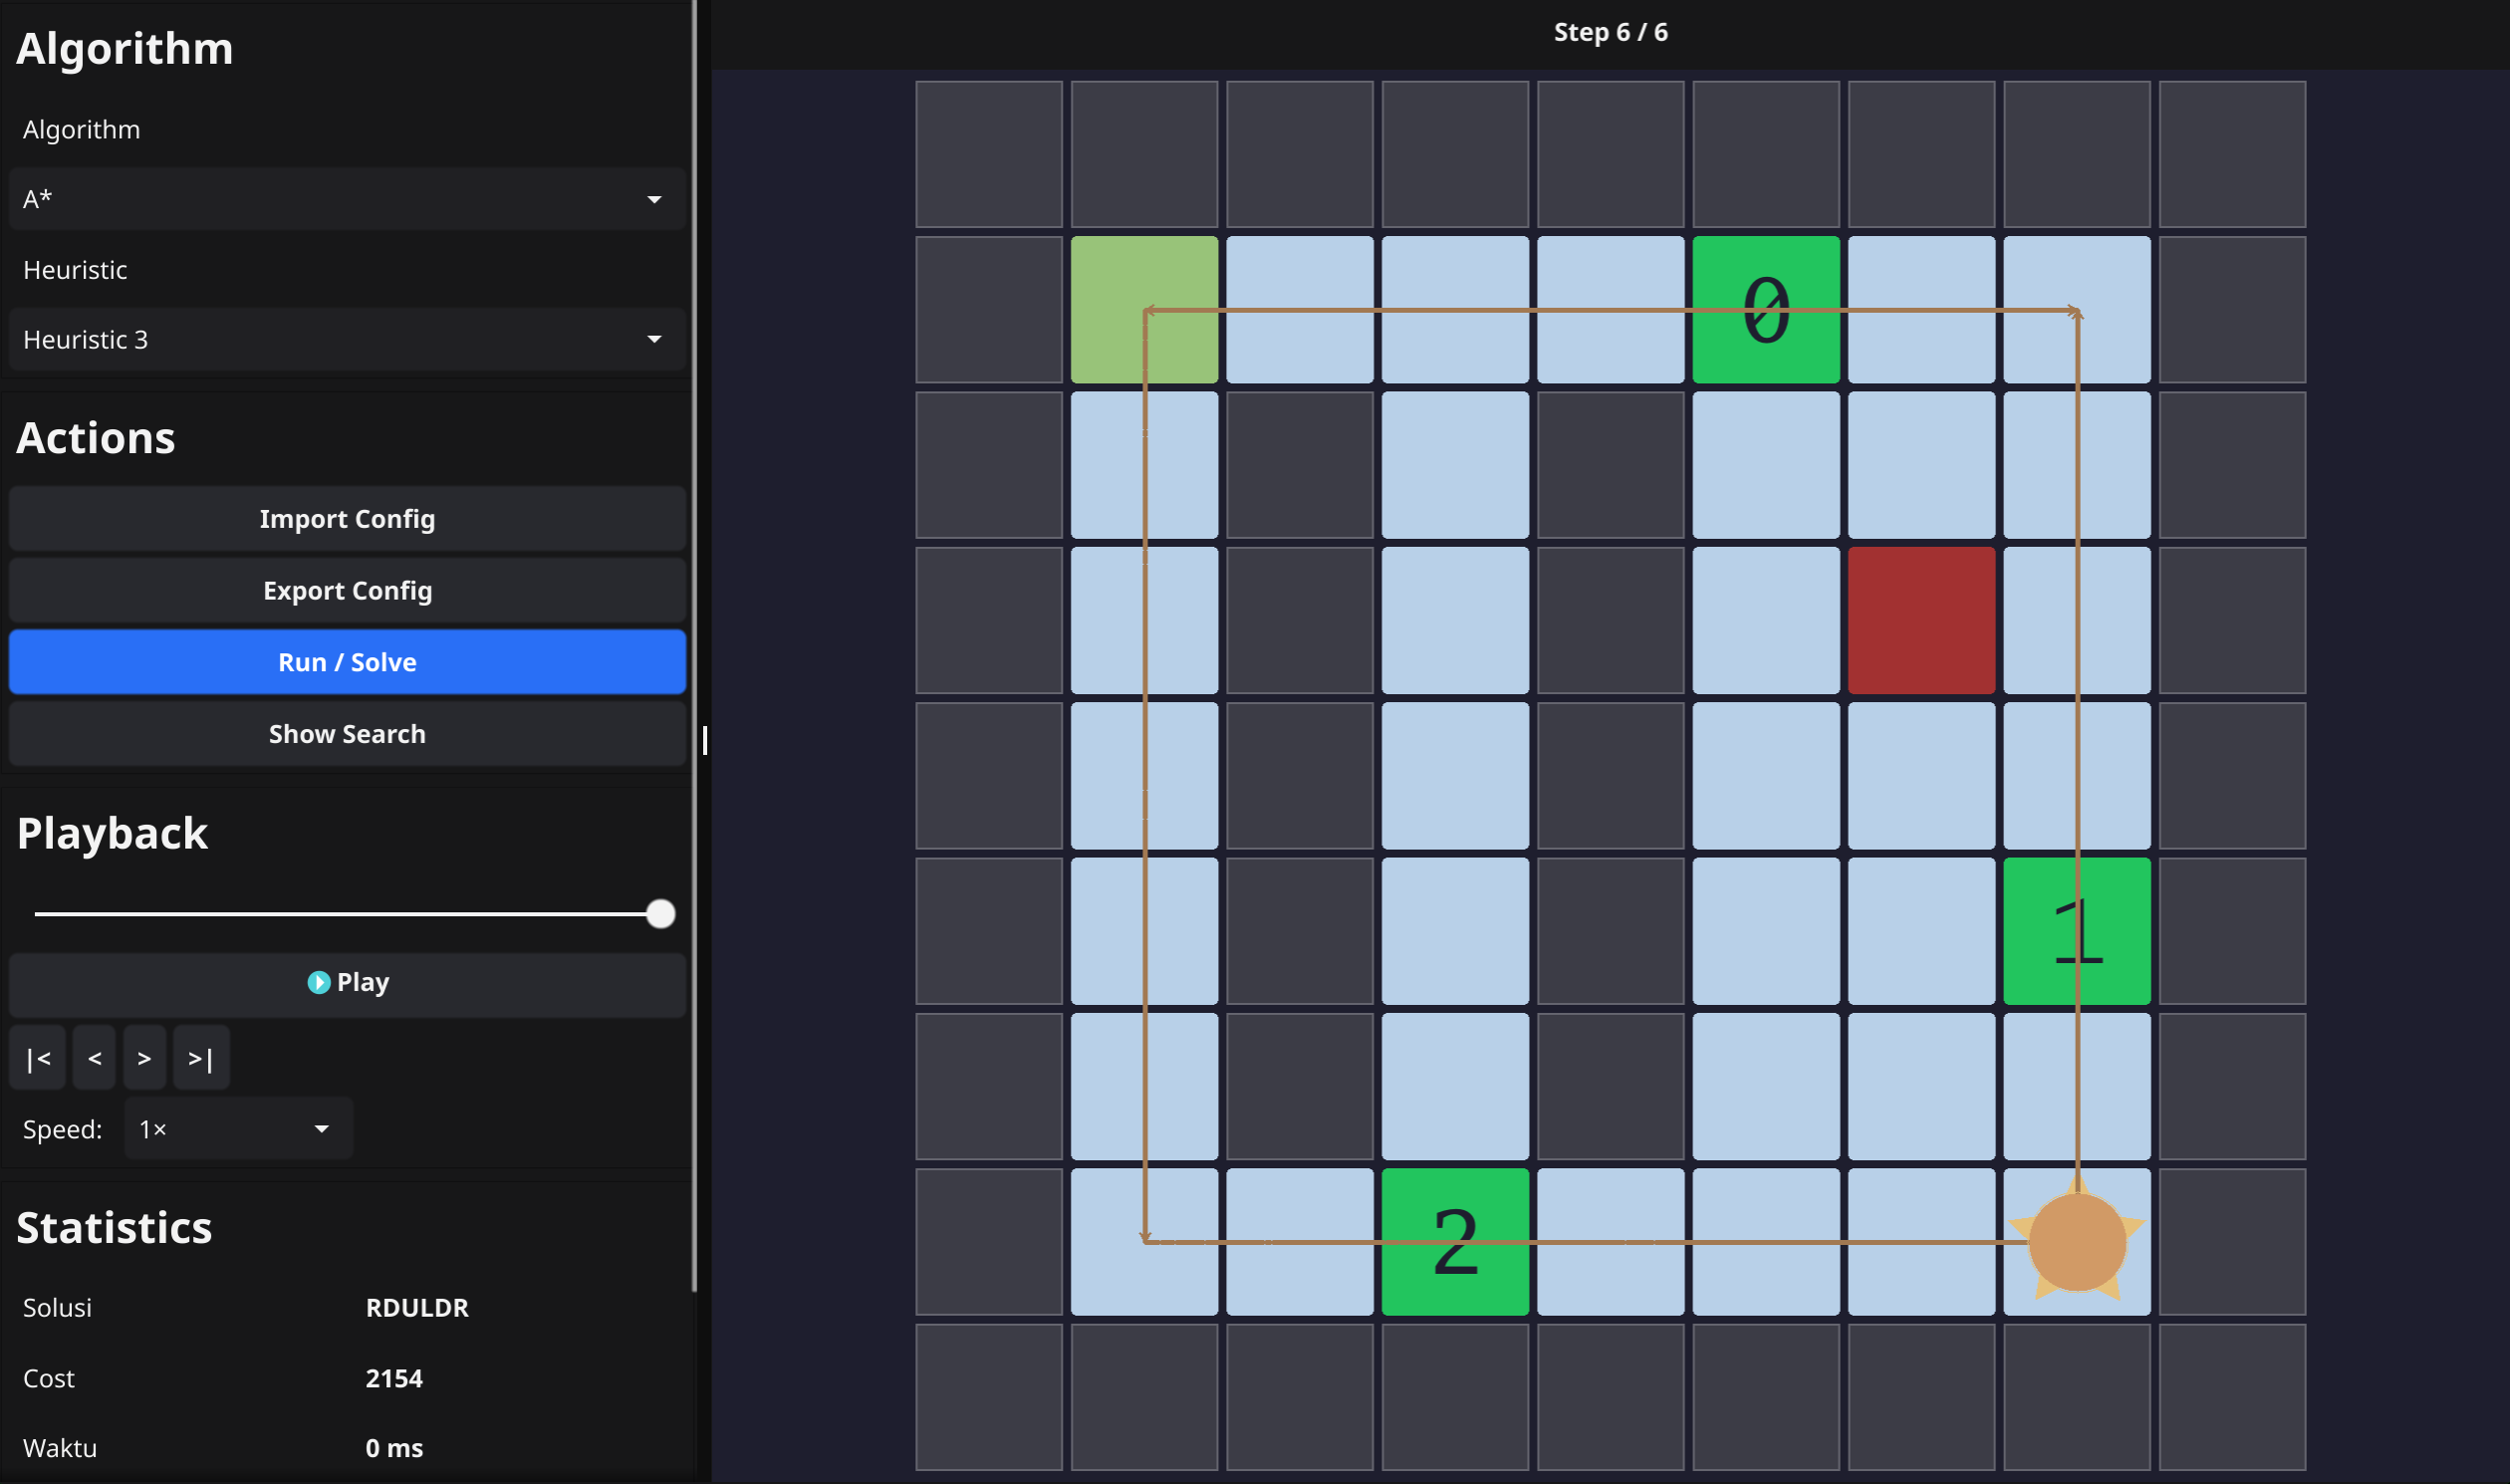
\includegraphics[width=0.8\textwidth]{astar_3.png}
  \caption{Hasil A* Heuristik 3 dengan input3.txt}
\end{figure}

\begin{tcolorbox}[title=\textbf{Hasil Pengujian}, colback=green!5!white, colframe=green!50!black]
\textbf{Solusi:} RDULDR\\
\textbf{Cost:} 2154\\
\textbf{Waktu:} 0 ms\\
\textbf{Iterasi:} 12
\end{tcolorbox}

\subsection{IDA* (Iterative Deepening A*) dengan input4.txt}

\subsubsection{IDA* Heuristik 1 dengan input4.txt}

\begin{figure}[H]
  \centering
  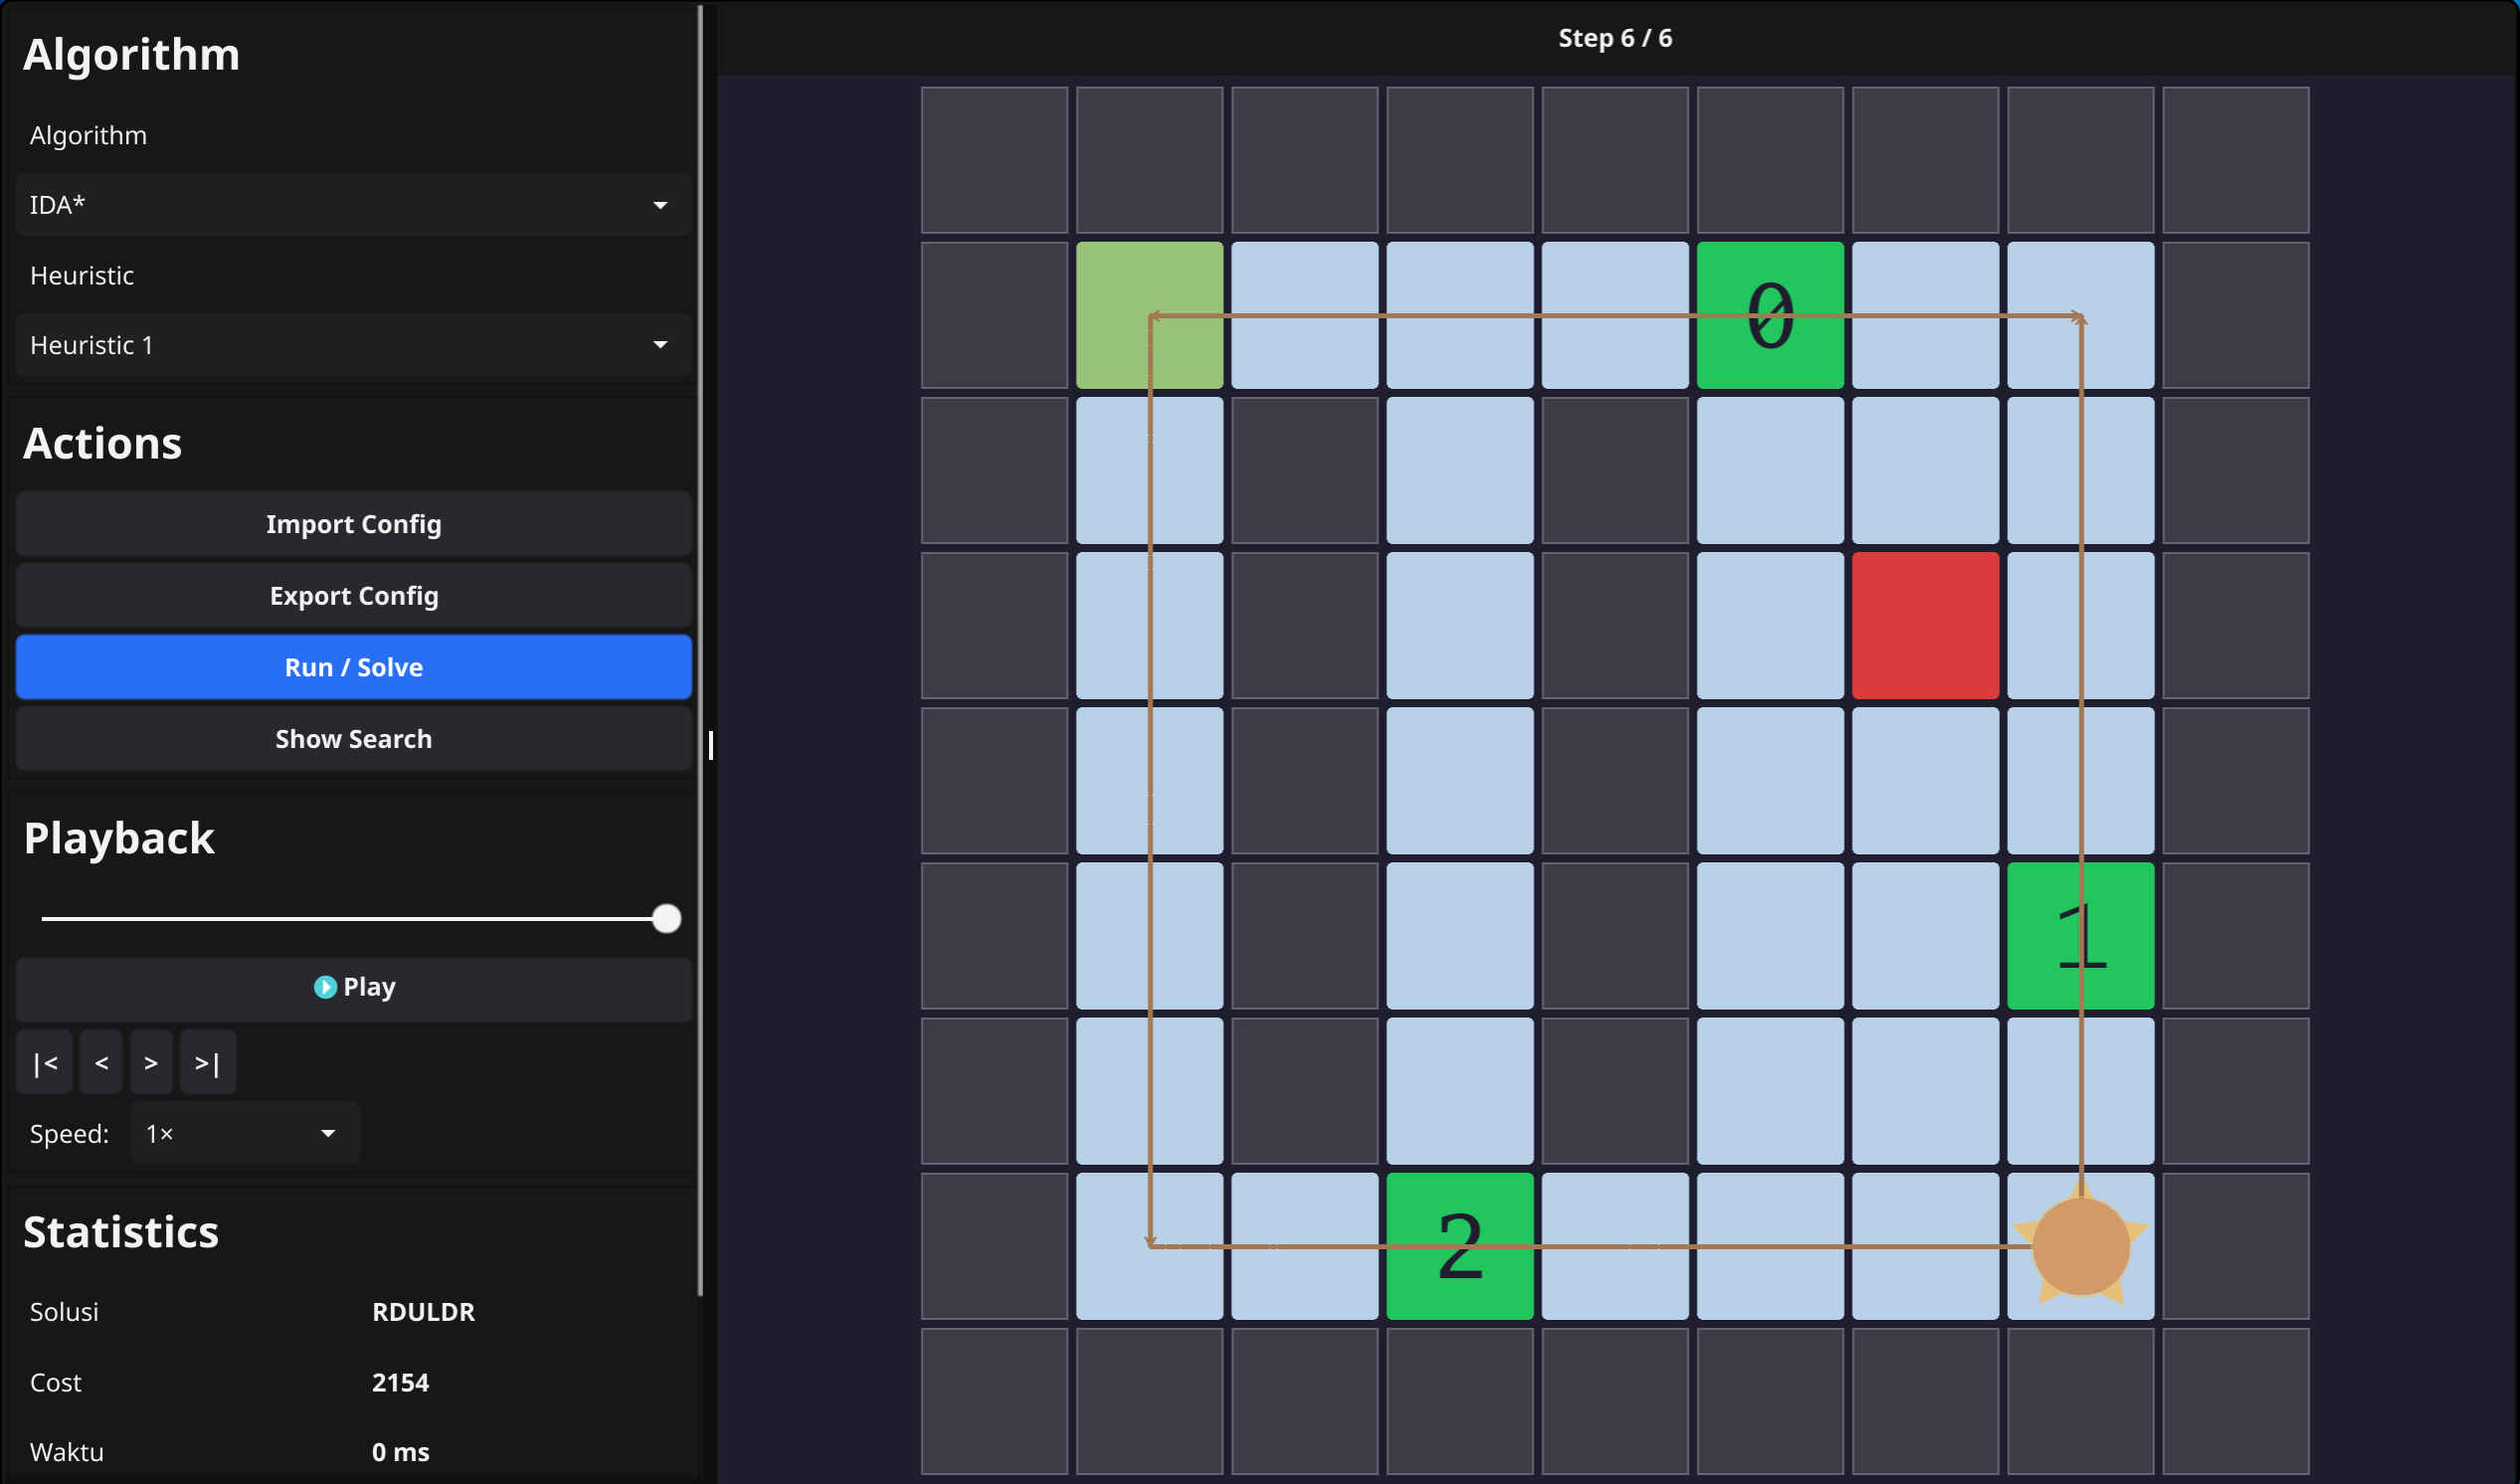
\includegraphics[width=0.8\textwidth]{idastar_1.png}
  \caption{Hasil IDA* Heuristik 1 dengan input4.txt}
\end{figure}

\begin{tcolorbox}[title=\textbf{Hasil Pengujian}, colback=green!5!white, colframe=green!50!black]
\textbf{Solusi:} RDULDR\\
\textbf{Cost:} 2154\\
\textbf{Waktu:} 0 ms\\
\textbf{Iterasi:} 91
\end{tcolorbox}

\subsubsection{IDA* Heuristik 2 dengan input4.txt}

\begin{figure}[H]
  \centering
  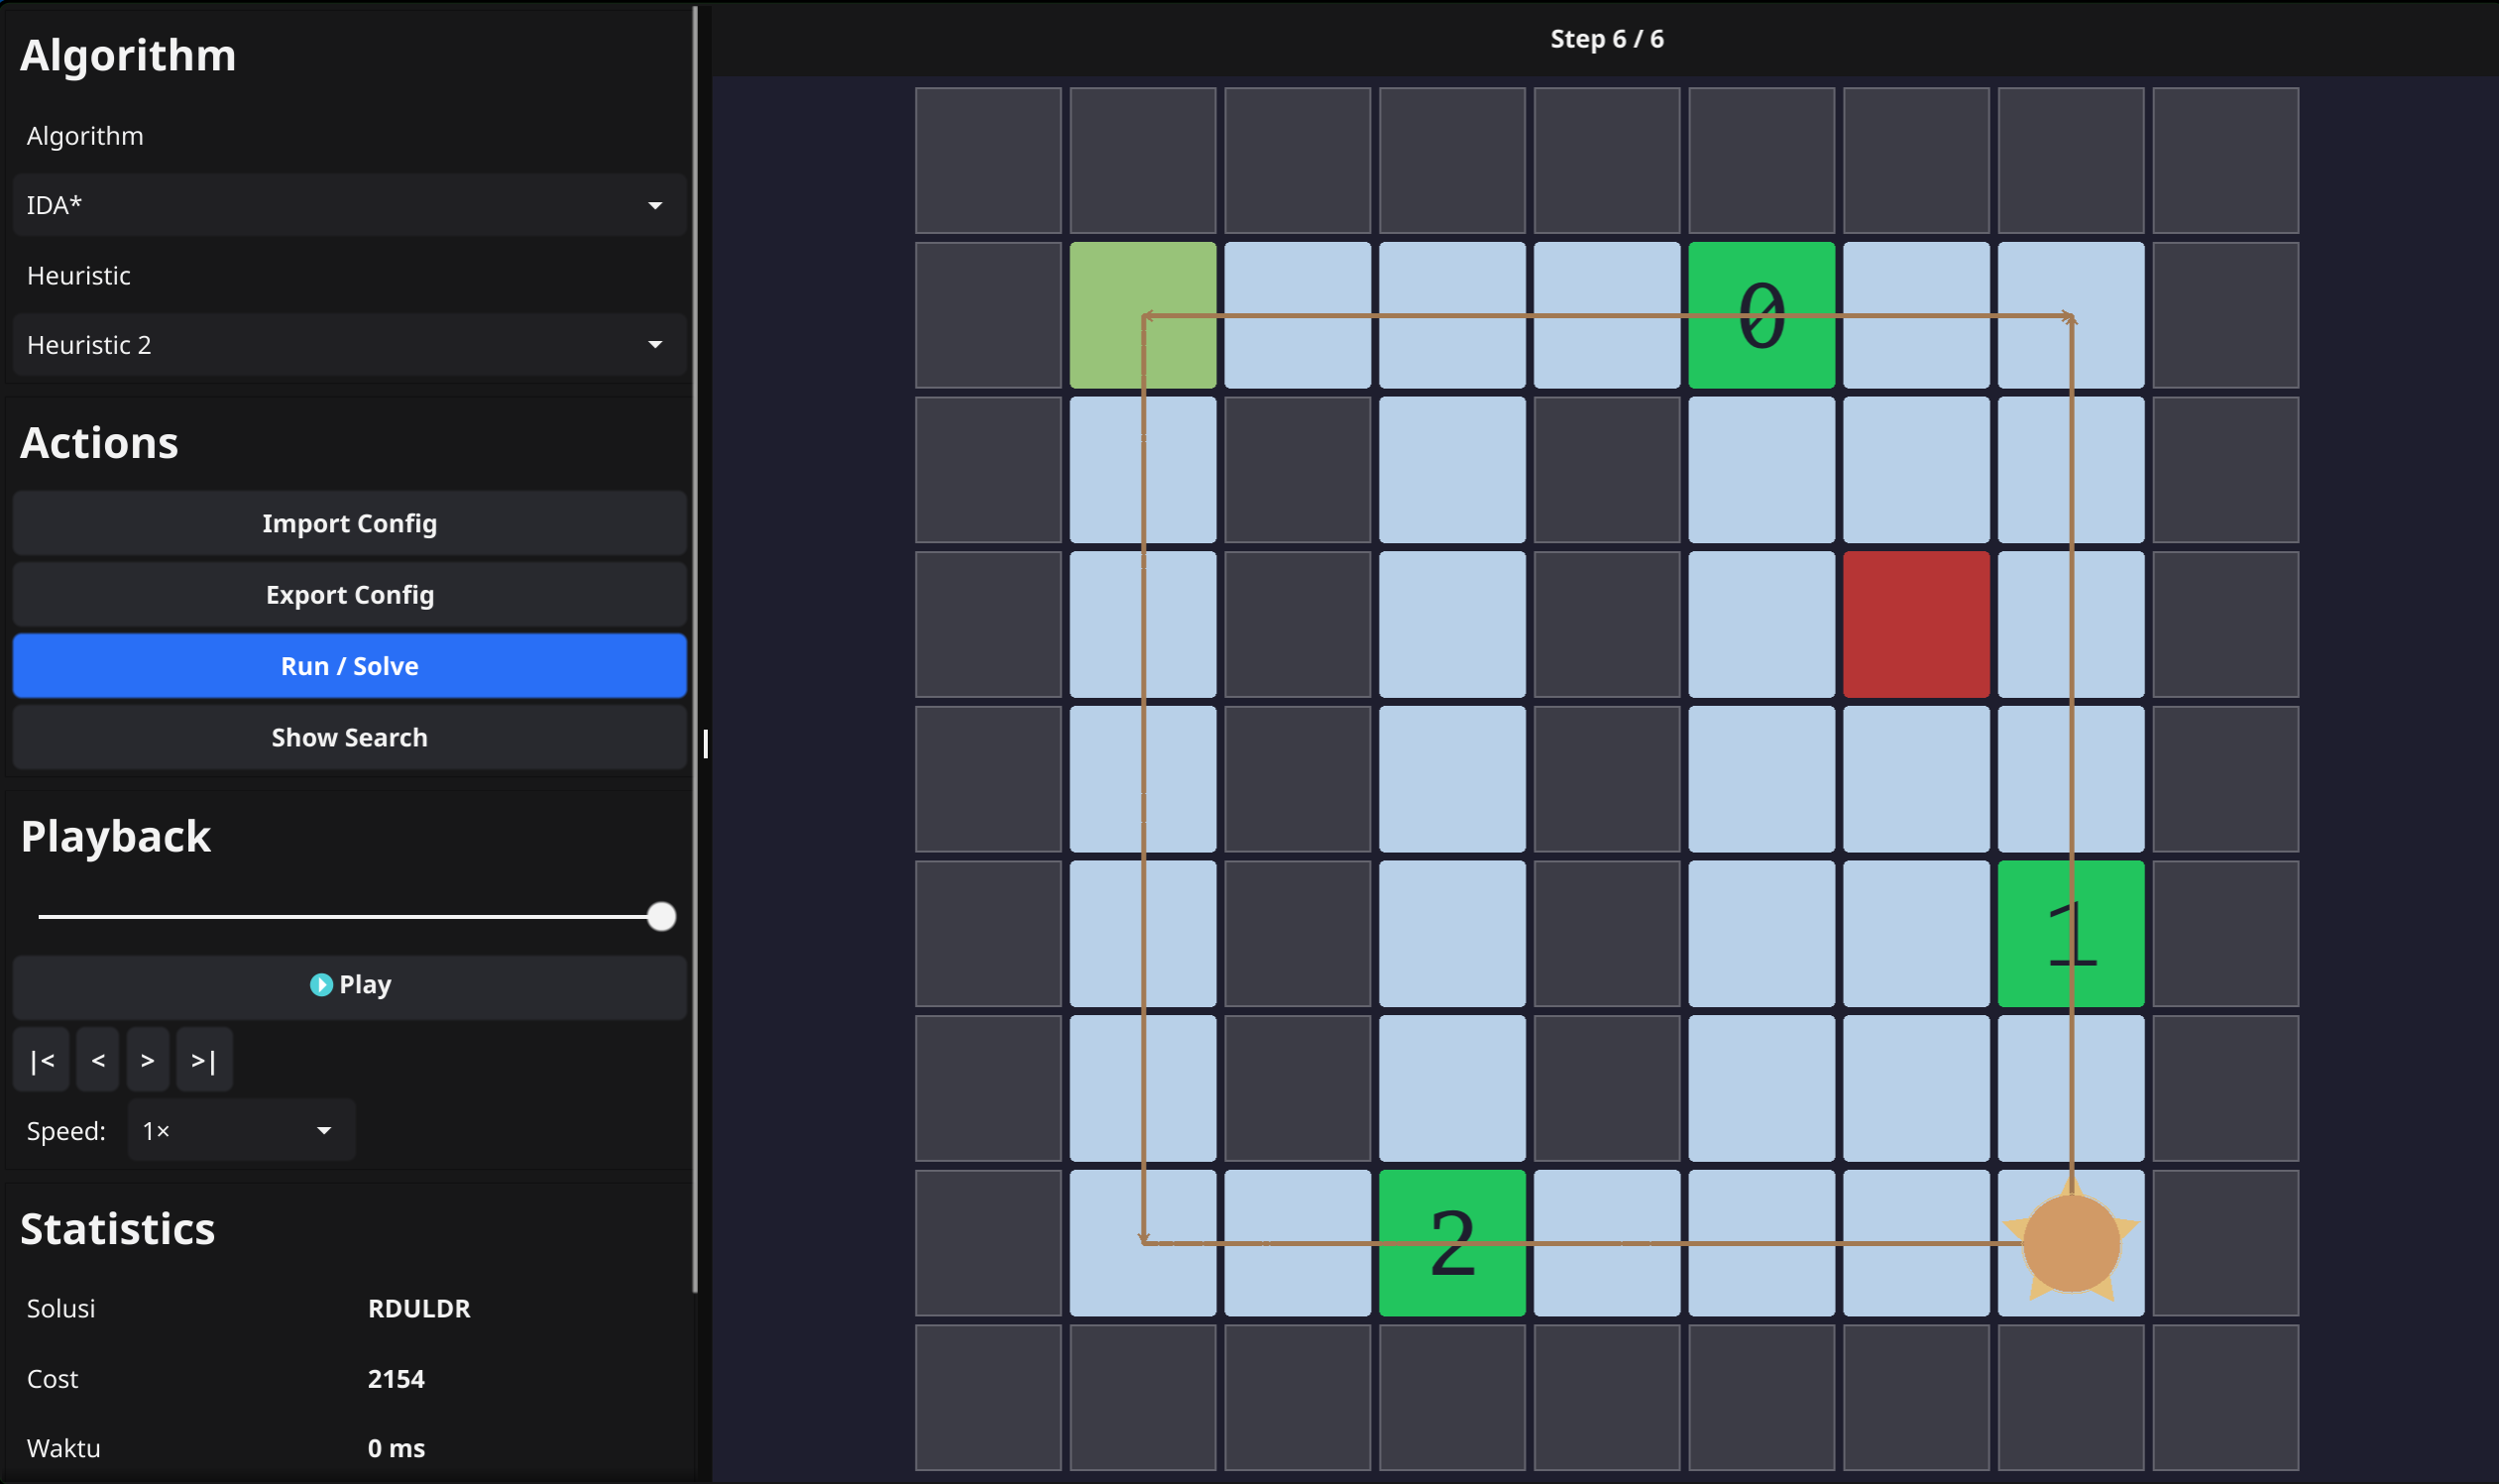
\includegraphics[width=0.8\textwidth]{idastar_2.png}
  \caption{Hasil IDA* Heuristik 2 dengan input4.txt}
\end{figure}

\begin{tcolorbox}[title=\textbf{Hasil Pengujian}, colback=green!5!white, colframe=green!50!black]
\textbf{Solusi:} RDULDR\\
\textbf{Cost:} 2154\\
\textbf{Waktu:} 0 ms\\
\textbf{Iterasi:} 91
\end{tcolorbox}

\subsubsection{IDA* Heuristik 3 dengan input4.txt}

\begin{figure}[H]
  \centering
  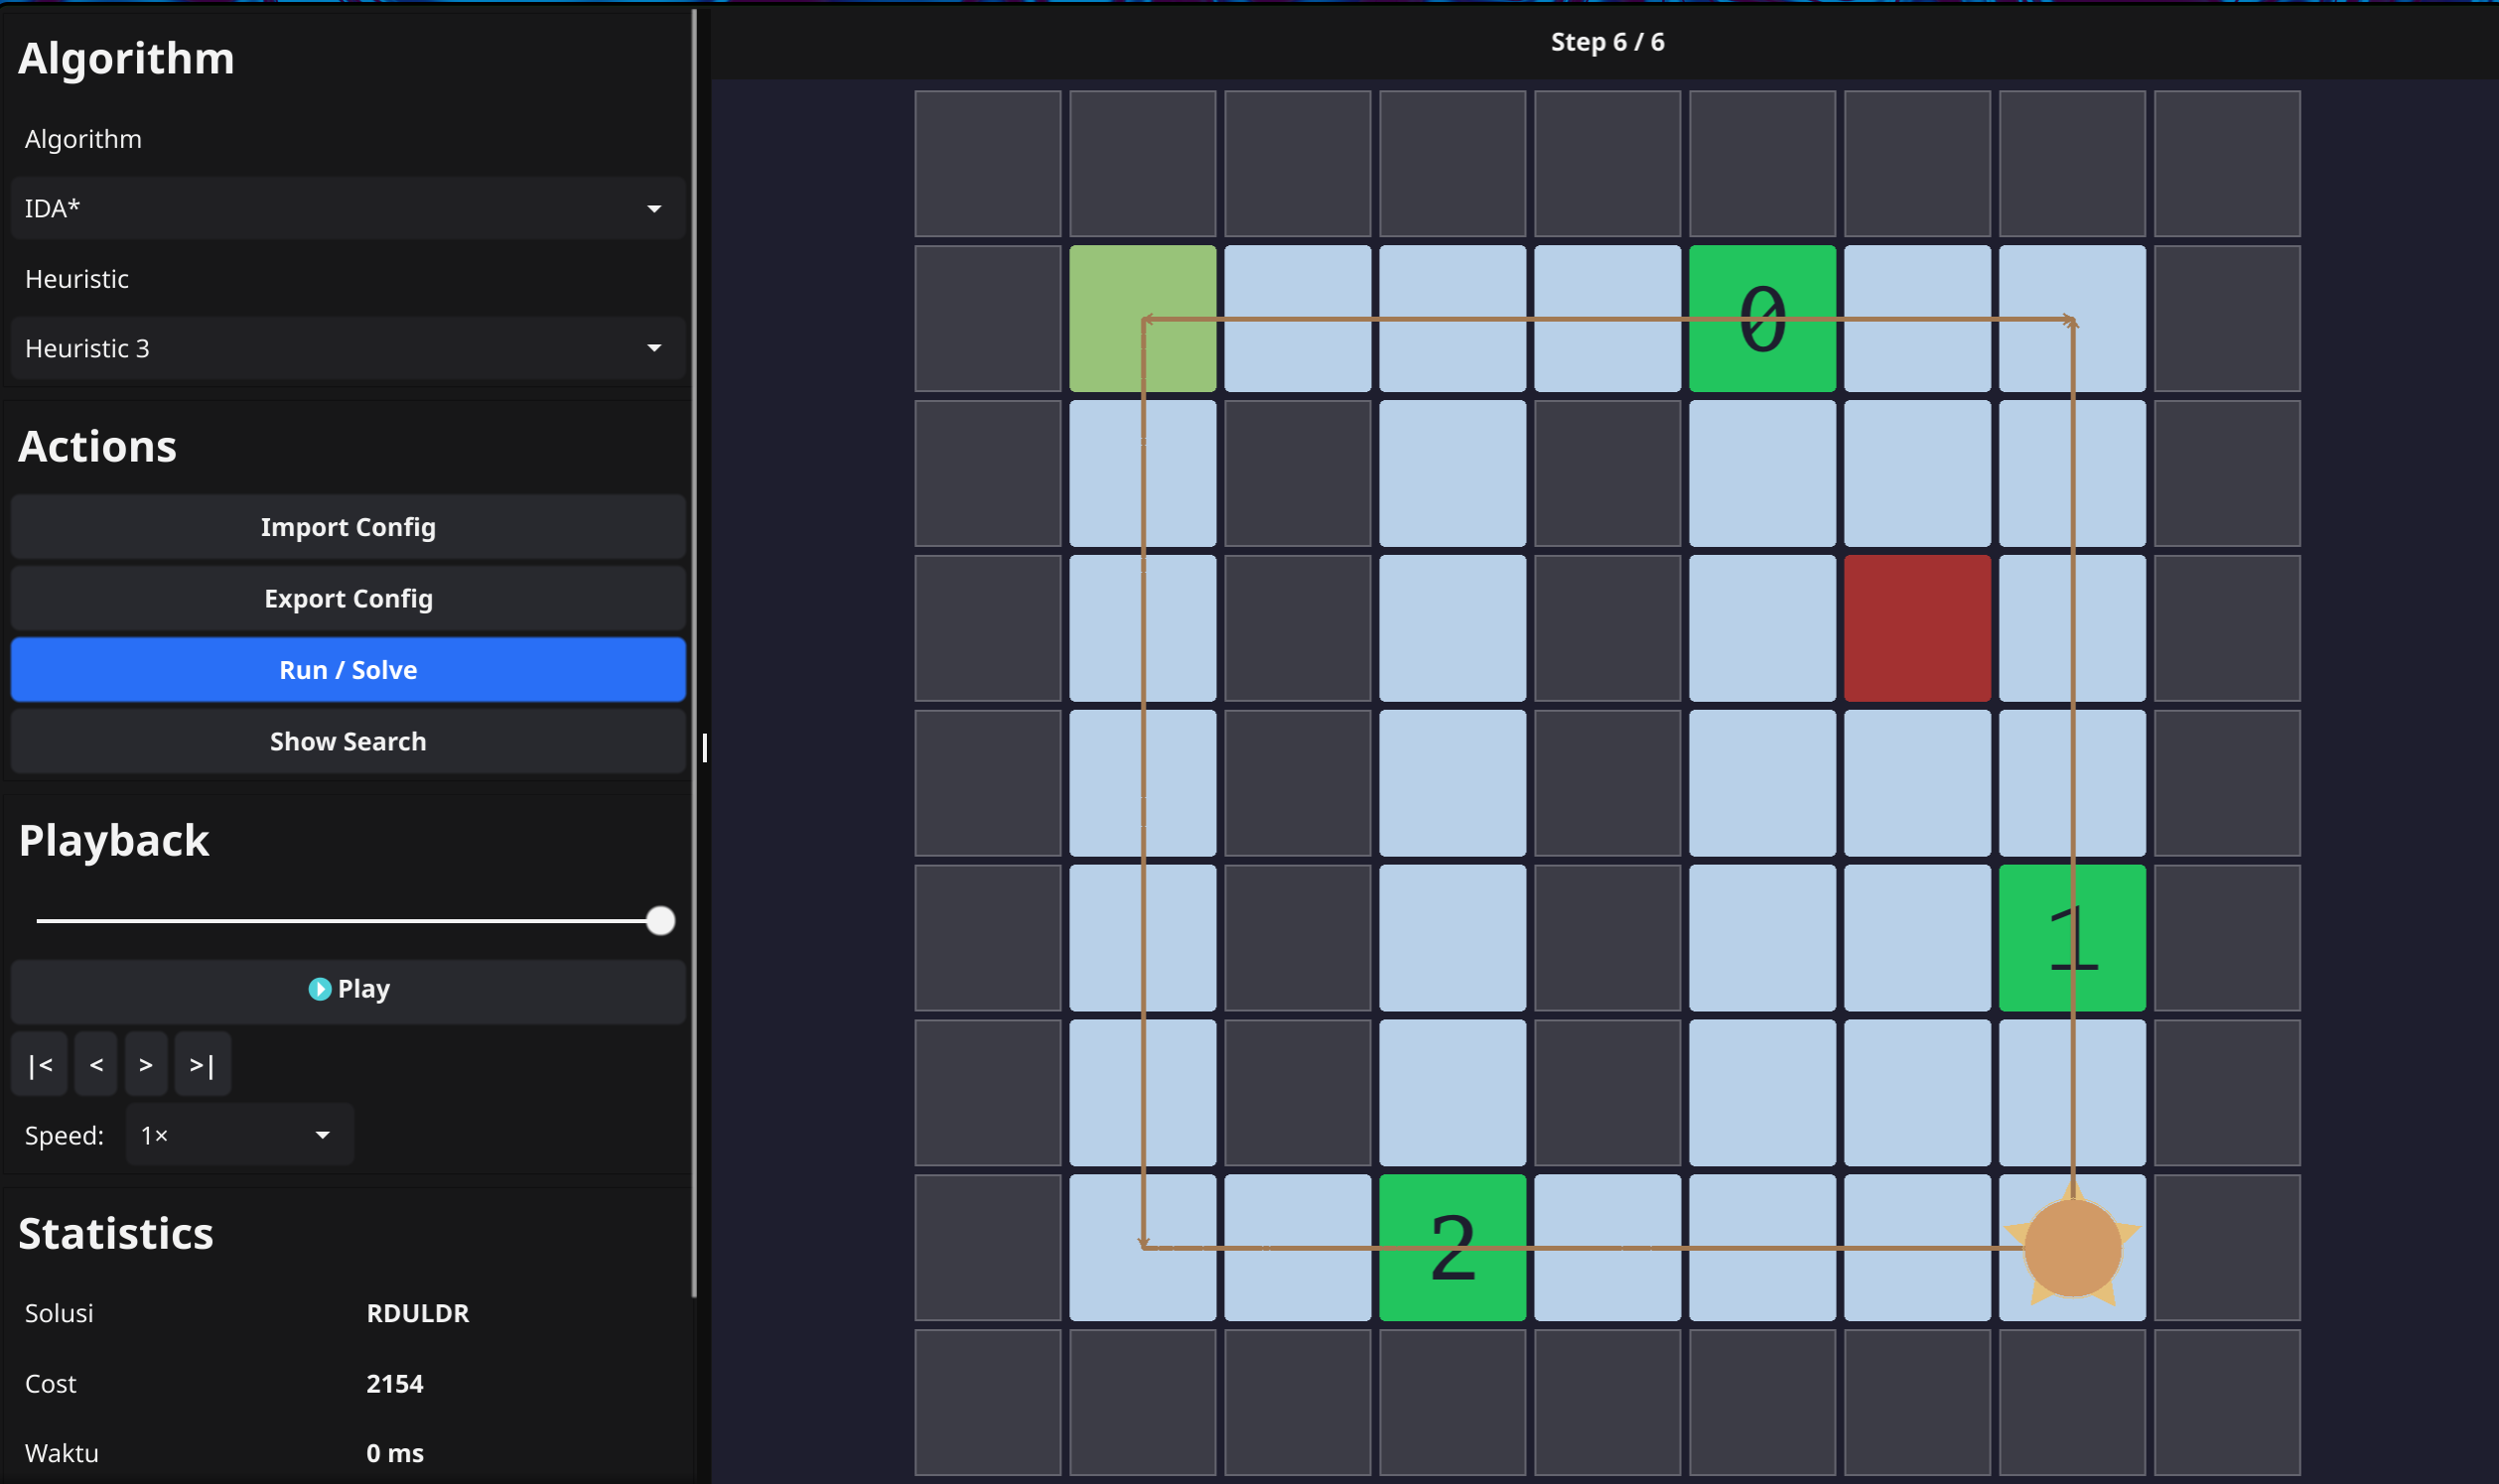
\includegraphics[width=0.8\textwidth]{idastar_3.png}
  \caption{Hasil IDA* Heuristik 3 dengan input4.txt}
\end{figure}

\begin{tcolorbox}[title=\textbf{Hasil Pengujian}, colback=green!5!white, colframe=green!50!black]
\textbf{Solusi:} RDULDR\\
\textbf{Cost:} 2154\\
\textbf{Waktu:} 0 ms\\
\textbf{Iterasi:} 91
\end{tcolorbox}

\subsection{Analisis Keseluruhan}

\subsubsection{Perbandingan Performa Algoritma}

\begin{table}[H]
    \centering
    \caption{Perbandingan Performa Algoritma pada Test Case}
    \label{tab:performance-compare}
    \begin{tabular}{|l|c|c|c|c|}
        \hline
        \textbf{Algoritma} & \textbf{Optimal} & \textbf{Waktu} & \textbf{Memori} & \textbf{Completeness} \\
        \hline
        UCS & Ya & Lambat & Tinggi & Ya \\
        \hline
        GBFS & Tidak & Cepat & Sedang & Ya* \\
        \hline
        A* & Ya** & Cepat & Sedang & Ya \\
        \hline
        IDA* & Ya** & Sedang & Rendah & Ya \\
        \hline
        \multicolumn{5}{l}{\footnotesize * Dengan visited set} \\
        \multicolumn{5}{l}{\footnotesize ** Dengan heuristik admissible} \\
    \end{tabular}
\end{table}

\subsubsection{Analisis Algoritma  UCS }

UCS menawarkan jaminan completeness dan optimalitas yang kuat, di mana algoritma ini selalu menemukan solusi dengan biaya minimum apabila solusi tersedia, tanpa bergantung pada fungsi heuristik sama sekali. Namun demikian, karakteristik UCS yang selalu mengekspansi node berdasarkan biaya kumulatif terkecil menyebabkan eksplorasi ruang keadaan yang sangat luas sebelum mencapai goal. Hal ini berimplikasi pada penggunaan memori yang tinggi karena seluruh frontier harus disimpan dalam priority queue, serta waktu eksekusi yang lambat terutama untuk papan berukuran besar dengan variasi biaya yang kompleks.

\subsubsection{Analisis Algoritma  GBFS }

GBFS menonjol dalam hal kecepatan eksekusi karena selalu memprioritaskan node dengan estimasi jarak terdekat ke goal tanpa memperhatikan biaya historis yang telah ditempuh. Strategi "rakus" ini memungkinkan algoritma untuk cepat menuju goal dalam banyak kasus. Akan tetapi, kelemahan fundamental GBFS adalah tidak adanya jaminan optimalitas solusi, sehingga sering kali menghasilkan jalur sub-optimal dengan biaya tinggi. Selain itu, GBFS rentan terjebak dalam jalur yang diarahkan oleh heuristik namun ternyata memiliki rintangan mematikan atau biaya traversal yang besar, serta sangat bergantung pada kualitas fungsi heuristik yang digunakan.

\subsubsection{Analisis Algoritma  A* }

A* berhasil menggabungkan keunggulan UCS dan GBFS melalui formulasi $f(n) = g(n) + h(n)$, sehingga mampu menjamin optimalitas solusi asalkan heuristik yang digunakan bersifat admissible, sambil tetap lebih efisien dalam eksplorasi node dibanding UCS. Kombinasi biaya aktual dan estimasi jarak memberikan keseimbangan yang ideal antara eksplorasi dan eksploitasi. Kendati demikian, A* tetap memiliki keterbatasan pada penggunaan memori yang tinggi untuk papan berukuran besar karena menyimpan seluruh frontier dan visited set, serta memerlukan fungsi heuristik yang baik untuk mencapai performa optimal.

\subsubsection{Analisis Algoritma IDA* }

IDA* menawarkan solusi yang sangat efisien dari sisi penggunaan memori dengan kompleksitas ruang linear terhadap kedalaman pencarian, karena tidak menyimpan frontier dalam struktur data eksplisit melainkan menggunakan rekursi DFS dengan threshold adaptif. Algoritma ini tetap menjamin optimalitas solusi dengan heuristik admissible dan tidak memerlukan priority queue. Namun demikian, mekanisme iterative deepening menyebabkan IDA* dapat melakukan re-ekspansi node yang sama di iterasi berbeda, yang pada beberapa kasus mengakibatkan waktu eksekusi lebih lambat dibanding A*, terutama ketika threshold harus sering diperbarui.


\section{Kesimpulan dan Saran}

\subsection{Kesimpulan}
\begin{enumerate}[label=\arabic*., leftmargin=2em]
  \item \textbf{UCS} menjamin solusi optimal namun memerlukan eksplorasi node yang sangat luas dan penggunaan memori yang tinggi. Algoritma ini cocok untuk kasus dengan biaya variatif yang signifikan.
  
  \item \textbf{GBFS} memberikan kecepatan eksekusi terbaik namun tidak menjamin optimalitas solusi. Heuristik 3 (checkpoint berantai) memberikan performa terbaik untuk kasus dengan angka berurutan.
  
  \item \textbf{A*} merupakan algoritma terbaik secara keseluruhan karena menjamin optimalitas dengan eksplorasi node yang lebih efisien dibanding UCS. Kombinasi $g(n) + h(n)$ memberikan keseimbangan ideal.
  
  \item \textbf{IDA*} sangat efisien dalam penggunaan memori (linear) namun dapat lebih lambat karena re-ekspansi node. Cocok untuk kasus dengan keterbatasan memori.
  
  \item Ketiga heuristik yang diimplementasikan (H1, H2, H3) bersifat \textit{admissible} dan dapat digunakan untuk menjamin optimalitas pada A* dan IDA*.
\end{enumerate}

\subsection{Saran Pengembangan}
\begin{enumerate}[label=\arabic*., leftmargin=2em]
  \item Implementasi heuristik tambahan yang lebih canggih seperti \textit{Pattern Database} untuk meningkatkan estimasi jarak.
  \item Optimisasi struktur data untuk mengurangi waktu eksekusi pada papan berukuran besar.
  \item Penambahan fitur visualisasi animasi gerakan aktor untuk memperjelas solusi.
  \item Implementasi algoritma pencarian paralel untuk memanfaatkan multi-core processor.
\end{enumerate}

\subsection{Refleksi Individu}

\subsubsection{\MemberA}
\textbf{Peran:} Implementasi struktur data utama, struktur dasar GUI, heuristik
kedua, dan GBFS. \\
\textbf{Pesan:} Semoga dapat dirancang sebuah heuristik route-finding untuk menghindari Viking
saat Persib menang, saya sendiri plat B hampir celaka

\subsubsection{\MemberB}
\textbf{Peran:} Implementasi heuristik 1 dan 3, UCS, A*, IDA*, dan pengembangan
GUI.\\
\textbf{Pesan:} Sa curi curi pandang. Kaka pu manis, bikin sa suka.

\newpage
\addcontentsline{toc}{section}{Referensi}
\section*{Referensi}

\begin{enumerate}[label={[\arabic*]}, leftmargin=2.5em, itemsep=0.3em]

\item N. U. Maulidevi, ``Penentuan Rute (\textit{Route/Path Planning}) Bagian 1:
      BFS, DFS, UCS, Greedy Best First Search,''
      Bahan Kuliah IF2211 Strategi Algoritma,
      Program Studi Teknik Informatika, STEI ITB, 2026.
      [Online]. Tersedia:
      \url{https://informatika.stei.itb.ac.id/~rinaldi.munir/Stmik/2025-2026/21-Route-Planning-(2026)-Bagian1.pdf}

\item N. U. Maulidevi dan R. Munir, ``Penentuan Rute (\textit{Route/Path Planning}) Bagian 2:
      Algoritma A*,''
      Bahan Kuliah IF2211 Strategi Algoritma,
      Program Studi Teknik Informatika, STEI ITB, 2026.
      [Online]. Tersedia:
      \url{https://informatika.stei.itb.ac.id/~rinaldi.munir/Stmik/2025-2026/22-Route-Planning-(2026)-Bagian2.pdf}

\item S. J. Russell dan P. Norvig, \textit{Artificial Intelligence: A Modern Approach},
      edisi ke-3. Upper Saddle River, NJ: Prentice-Hall International, 2010.

\item R. E. Korf, ``Depth-first iterative-deepening: An optimal admissible tree search,''
      \textit{Artificial Intelligence}, vol.~27, no.~1, hal.~97--109, 1985.
      \url{https://doi.org/10.1016/0004-3702(85)90084-0}

\end{enumerate}

\newpage
\section*{Lampiran}
\addcontentsline{toc}{section}{Lampiran}

\begin{enumerate}
    \item \textbf{Repositori GitHub:} \\
    \url{https://github.com/nicholaswisee/Tucil3_13524037_13524056}

    \item \textbf{Tabel Checklist Pembuatan Fitur:}

    \begin{table}[H]
        \centering
        \renewcommand{\arraystretch}{1.5}
        \begin{tabular}{|c|p{10cm}|c|c|}
            \hline
            \textbf{No} & \textbf{Poin} & \textbf{Ya} & \textbf{Tidak} \\
            \hline
            1 & Program berhasil dikompilasi tanpa kesalahan & \checkmark & \\
            \hline
            2 & Program berhasil dijalankan & \checkmark & \\
            \hline
            3 & Solusi yang diberikan program benar dan mematuhi aturan permainan & \checkmark & \\
            \hline
            4 & Program dapat membaca masukan berkas \texttt{.txt} serta menyimpan solusi dalam berkas \texttt{.txt} & \checkmark & \\
            \hline
            5 & Program memiliki \textit{Graphical User Interface} (GUI) & \checkmark & \\
            \hline
            6 & Ada algoritma \textit{pathfinding} alternatif selain dari spesifikasi wajib (IDA*) & \checkmark & \\
            \hline
            7 & Ada tambahan dua alternatif heuristik selain yang utama (H1 dan H3) & \checkmark & \\
            \hline
        \end{tabular}
        \caption{Tabel checklist implementasi fitur Tugas Kecil 3.}
        \label{tab:checklist}
    \end{table}

    \addcontentsline{toc}{section}{Pernyataan Keaslian}
    \item \textbf{Pernyataan Keaslian}
\end{enumerate}

\vspace{0.5cm}
\begin{center}
    \fbox{
        \begin{minipage}{0.9\linewidth}
            \vspace{0.3cm}
            \textbf{Pernyataan} \\
            
            Tugas ini disusun sepenuhnya tanpa bantuan kecerdasan buatan (\textit{Generative AI}), melainkan hasil pemikiran dan analisis mandiri.
            
            \vspace{1cm}
            \begin{minipage}{0.45\linewidth}
                \centering
                
\includegraphics[height=2.5cm]{ttd-wise.png} \\
                \vspace{0.2cm}
                Nicholas Wise Saragih S \\
                13524037
            \end{minipage}
            \hfill
            \begin{minipage}{0.45\linewidth}
                \centering
                
\includegraphics[height=2.5cm]{ttd-ponso.png} \\
                \vspace{0.2cm}
                Reinhard Alfonzo Hutabarat \\
                13524056
            \end{minipage}
            \vspace{0.3cm}
        \end{minipage}
    }
\end{center}

\end{document}
